\documentclass[11pt,a4paper]{article}
\usepackage[margin=2.2cm]{geometry}
\usepackage[T1]{fontenc}
\usepackage{lmodern}
\usepackage{booktabs}
\usepackage{graphicx}
\usepackage{amsmath}
\usepackage{xcolor}
\usepackage{caption}
\usepackage{subcaption}
\usepackage{hyperref}
\usepackage{enumitem}
\usepackage{float}
\usepackage{verbatim}
\usepackage[most]{tcolorbox}
\hypersetup{colorlinks=true, linkcolor=blue!50!black, urlcolor=blue!50!black, citecolor=blue!50!black}
\graphicspath{{figures/}}
\setlist{nosep}

% Model-generated text is always shown in this box, verbatim and unedited.
\newtcolorbox{modelout}[1]{colback=gray!6, colframe=gray!45, boxrule=0.4pt, arc=1pt, left=4pt, right=4pt,
  top=2pt, bottom=2pt, fonttitle=\footnotesize\bfseries, coltitle=black, colbacktitle=gray!18,
  title={MODEL OUTPUT (unedited) --- #1}}
\newcommand{\human}[1]{\textit{#1}}
\newcommand{\pending}[1]{\textcolor{red}{\textbf{[PENDING HUMAN RATINGS:} #1\textbf{]}}}

\title{\textbf{The Plot-Twist Generator}\\[2pt]
\large Can a small neural language model write an interesting story?\\
\normalsize NLP Group Assignment 2 --- Question 4}
\author{Paritosh Lahre (12341550)}
\date{3 November 2026}

\begin{document}
\maketitle

\begin{abstract}
We train a Vanilla RNN and an LSTM word-level language model from scratch on 20,000 TinyStories.
We use them to continue story openings with ten decoding configurations (greedy, temperature,
top-$k$, top-$p$ and a repetition penalty). We measure perplexity, diversity (Distinct-1/2),
repetition and length failures. We also run a blinded rating study of plot-twist continuations.
A human study was not possible in the time we had, so three LLM judges take the place of human evaluators.
We use a zero-shot Qwen2.5-0.5B-Instruct as an optional reference. The LSTM is clearly the better language model (test perplexity 11.81 vs.\ 15.77). It is
also the more stable generator. It has fewer repetition loops, and its story lengths are better calibrated.
Still, neither model tells the story it is asked to tell. In 50--68\% of samples, the continuation
reuses none of the opening's content words. Out-of-vocabulary words erase key parts of the premise. With a fixed
random seed, two different openings often give nearly the same continuation. Three blinded LLM
judges, used in place of human raters, give both models equally low scores (coherence 1.4 of 5). They see no
LSTM advantage. Lower perplexity brought fluency, not better storytelling.
\end{abstract}

\section{Introduction}
The brief asks two questions. Can a small neural language model write a story that is coherent,
interesting and surprising? And is the better language model (lower perplexity) also the
better storyteller? We answer with controlled experiments. The two architectures differ only in
the recurrent cell. They share one vocabulary and one training recipe. Every comparison uses the same
prompts, decoding settings and seeds. All generated text in this report appears
\emph{exactly} as the model produced it (we only detokenised the saved tokens). Model output always appears in
grey ``MODEL OUTPUT'' boxes. All other text is human commentary. We report failed generations
next to successful ones. The submission includes code, configuration, checkpoints and all raw generations
(see the README for exact commands).

\section{Data preparation and next-token prediction (Part 1)}
\label{sec:data}
\paragraph{Corpus and subset.} We stream the first 40,000 stories of the TinyStories
\texttt{train} split (\texttt{roneneldan/\allowbreak TinyStories}) in their published order. We clean them,
drop stories shorter than 20 words, and remove exact duplicates (ignoring case and whitespace).
We shuffle the unique stories with seed 42. Then we split them \emph{at the story level} into 20,000
training, 1,000 validation and 1,000 test stories. Only after this do we build training sequences. So no
part of a story can appear in more than one split. We save the Hugging Face row index of every story
in \texttt{data/splits.json}. The dataset itself is not part of the submission.
Table~\ref{tab:data} summarises the result.

\paragraph{Cleaning.} We apply Unicode NFKC normalisation. We repair wrongly decoded UTF-8 sequences that occur
in TinyStories (e.g.\ the three garbage characters left by a wrongly decoded apostrophe). We map curly quotes and dashes to ASCII.
We remove any remaining non-ASCII characters. We collapse repeated whitespace.

\paragraph{Tokenisation and vocabulary.} Both models share one word-level tokenizer. It
lowercases the text. Then a regular expression splits it into words, clitics (short attached word parts such as \texttt{'s}, \texttt{'t},
\texttt{'ll}, \dots), numbers and single punctuation marks. We build the vocabulary from the
\emph{training split only}. It keeps every token seen at least 3 times. Rarer tokens map to
\texttt{<unk>}. We add four special tokens: \texttt{<pad>} (id 0), \texttt{<unk>},
\texttt{<bos>} and \texttt{<eos>}.

\paragraph{Sequences and input--target pairs.} Every story becomes one id sequence
\texttt{<bos>} $w_1 \dots w_n$ \texttt{<eos>}. The model input is this sequence without its last id.
The target is the same sequence shifted left by one. So at every position $t$, the model predicts
$w_{t+1}$ from $w_{\le t}$ (example in Appendix~\ref{app:pairs}). Some stories are longer than 512 tokens
(Table~\ref{tab:data}). We cut these into consecutive windows of the \emph{same} story. The windows overlap by one
token, so every target is predicted exactly once. Hidden states start from zero for every window.

\paragraph{Why we keep story boundaries.} (i)~\emph{No leakage}: suppose overlapping windows
of one story could fall into different splits. Then validation and test perplexity would measure
memorisation, not generalisation. Splitting whole stories, after removing duplicates,
prevents this. (ii)~\emph{Correct conditioning}: suppose stories were joined into one stream. Then the
model would learn to continue the end of story A with the start of an unrelated story B. The
hidden state would also carry characters and events across the boundary. (iii)~\emph{Learning to
stop}: the model can learn when a story is finished only if every story ends with an explicit \texttt{<eos>}.
Our premature-termination and runaway metrics (Part~5) depend on this.

\paragraph{Padding.} We group windows into batches of similar length (about 12k tokens per
batch). We right-pad them with \texttt{<pad>}. \texttt{ignore\_index} removes padded target positions
from the loss. Both models are causal: they read left to right. So padding placed after
the real tokens cannot change any hidden state or prediction at a real position. The loss therefore
equals the loss on the unpadded sequences. The pad embedding is fixed at zero
(\texttt{padding\_idx}).

\begin{table}[H]\centering\small
\caption{Data statistics.}\label{tab:data}
\begin{tabular}{ll}
\toprule
Quantity & Value \\
\midrule
Stories streamed (HF train, in order) & 40000 \\
Dropped: too short / exact duplicates & 12 / 50 \\
Train / val / test stories & 20000 / 1000 / 1000 \\
Train tokens & 4,221,472 \\
Word types in train / vocabulary size & 10,971 / 7,590 \\
Train tokens covered by vocabulary & 99.90\% \\
\texttt{<unk>} rate val / test & 0.20\% / 0.22\% \\
Mean / max train story length (tokens) & 213 / 1025 \\
Train stories split into >1 window & 531 (2.65\%) \\
\bottomrule
\end{tabular}

\end{table}

\section{Models and training (Part 2)}
\label{sec:models}
\paragraph{Architectures.} Model A: \texttt{Embedding(V,256)} $\rightarrow$ 2-layer
\texttt{nn.RNN} (tanh, hidden 512) $\rightarrow$ \texttt{Linear(512,V)}. Model B is the same, but
uses \texttt{nn.LSTM} instead of \texttt{nn.RNN}. We apply dropout 0.3 to the embeddings, between
the recurrent layers and before the output layer. We train both models with token-level cross-entropy.

\paragraph{Same training conditions.} Both models use the same data, vocabulary, batches (seed 42),
embedding and hidden sizes, depth and dropout. We use AdamW (lr $10^{-3}$, weight decay 0.01) and
clip the gradient norm at 1.0. ReduceLROnPlateau (factor 0.5) lowers the learning rate when the
validation loss stops improving. Training runs for at most 15 epochs, with early stopping
(patience 2). We keep the checkpoint with the lowest validation loss. We train with mixed precision
(bf16 autocast) on one NVIDIA RTX 3050 Ti Laptop GPU (4~GB).
\emph{Unavoidable difference}: an LSTM layer has four gates. So it has four times the recurrent
weights of a Vanilla RNN layer of the same width. As a result, the LSTM has more parameters
(Table~\ref{tab:models}). We kept the widths equal, as the brief asks. We did not match the
parameter counts.

\begin{table}[H]\centering\small
\caption{Model size, training cost and perplexity. Perplexity = exp of the mean token-level
cross-entropy over all non-pad targets, including \texttt{<eos>}.}\label{tab:models}
\resizebox{\linewidth}{!}{\begin{tabular}{lllrrlll}
\toprule
Model & Params (total) & Recurrent params & Epochs run & Best epoch & Train time (min) & Val PPL & Test PPL \\
\midrule
Vanilla RNN & 6.76M & 0.92M & 15 & 15 & 5.4 & 16.00 & 15.77 \\
LSTM & 9.51M & 3.68M & 15 & 15 & 7.5 & 11.99 & 11.81 \\
\bottomrule
\end{tabular}
}
\end{table}

\begin{figure}[H]\centering
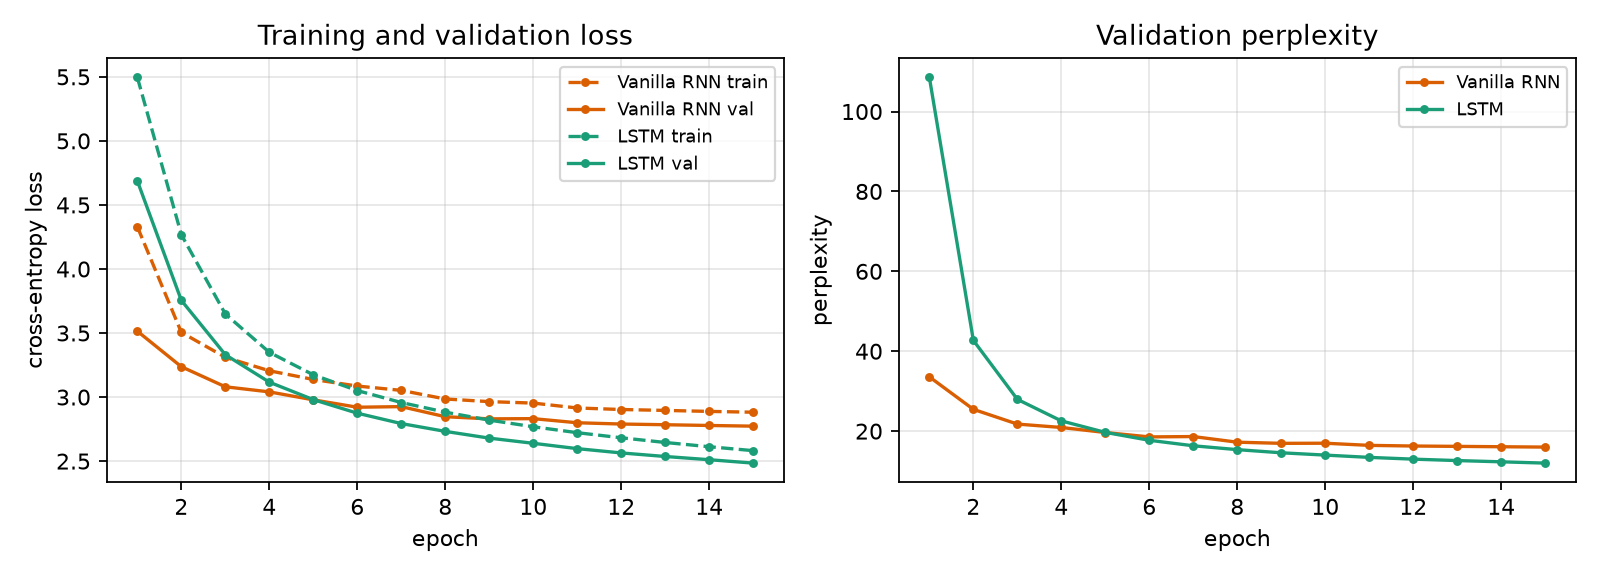
\includegraphics[width=\linewidth]{loss_curves.png}
\caption{Training and validation loss per epoch, and validation perplexity.}\label{fig:loss}
\end{figure}

\paragraph{Results.} With the same width and training budget, the LSTM reaches 25\% lower
perplexity than the Vanilla RNN. This holds on both validation and test data (Table~\ref{tab:models}).
The RNN learns faster at first. After epoch~1, its validation perplexity is 33.6, while the LSTM's
is 108.6. The LSTM has more parameters and has to learn its gates. The curves cross between
epochs~5 and~6 (19.65 vs.\ 19.68, then 18.55 vs.\ 17.71). After that, the LSTM keeps improving
faster (Fig.~\ref{fig:loss}). Neither model had fully converged (stopped improving) within the
15-epoch budget. In the last epoch, validation perplexity still fell from 16.09 to 16.00 (RNN) and
from 12.32 to 11.99 (LSTM). The LSTM curve is steeper. This suggests that the gap would grow with
longer training. For both models, training loss is higher than validation loss. This is because
dropout is active only during training.

\paragraph{Gradient behaviour.} Before clipping, the RNN's gradient norm jumped as high as 39.
In 1.8\% of the logged steps, it was above the clipping threshold of 1.0. The LSTM's gradient norm
never went above 1.62 (Fig.~\ref{fig:grad}). This is the exploding-gradient behaviour (sudden, very
large gradients) that we expect from a tanh RNN. Such a model is trained by backpropagation through
time over hundreds of steps. Gradient clipping kept the RNN's training stable.

\paragraph{Loss by position.} Fig.~\ref{fig:grad} (right) shows the test loss at each token position
in the story. Both models find the first tokens easy (``once upon a time''). So the curve itself
mostly reflects the structure of the stories. The useful number is the \emph{gap} between the two
models. The LSTM's advantage is 0.04 nats on the first 8 tokens and 0.23 on tokens 8--32. From
token 32 onwards, it is about 0.31 (0.30 for positions 256--512). So the LSTM gains little where
there is little context, and a lot where there is more. This is the typical sign of a model that
keeps information from further back. Gating is designed to do this.

\begin{figure}[H]\centering
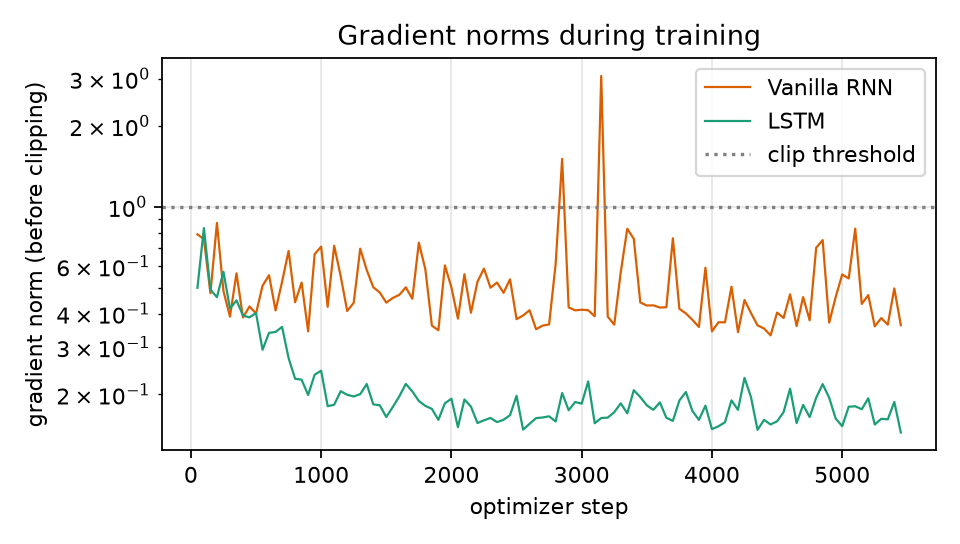
\includegraphics[width=0.49\linewidth]{grad_norms.png}\hfill
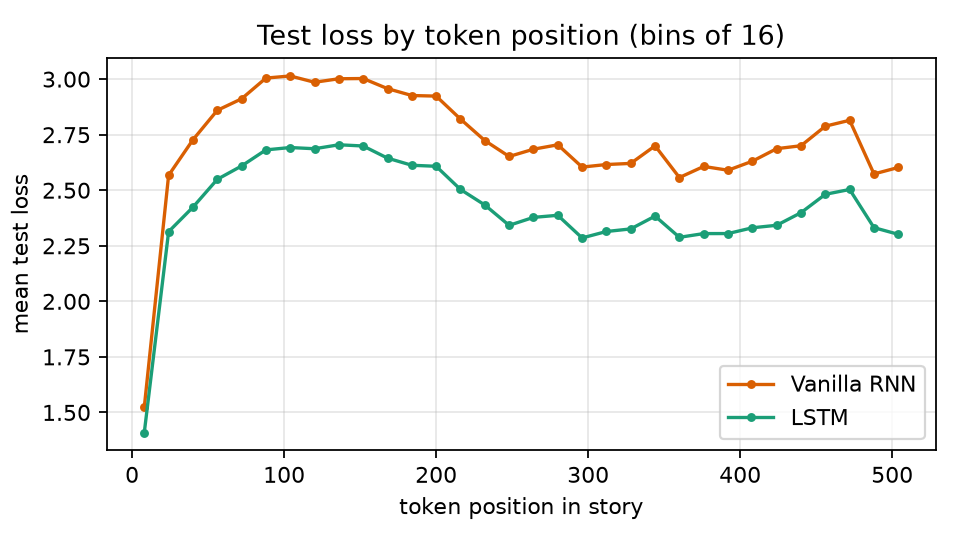
\includegraphics[width=0.49\linewidth]{loss_by_position.png}
\caption{Left: gradient norm before clipping (log scale). Right: mean test loss by token position
(16-token bins; bins with $<$200 tokens are left out).}\label{fig:grad}
\end{figure}

\section{Decoding strategies (Part 3)}
\label{sec:decoding}
For each prompt, we encode \texttt{<bos>} + prompt and run it through the model. Then we generate
up to 150 tokens, one at a time, and feed the hidden state back at each step. We stop at
\texttt{<eos>}. At every step we mask out \texttt{<unk>}, \texttt{<pad>} and \texttt{<bos>}, so
the model cannot generate them.
We use these strategies:
\begin{itemize}
\item \textbf{Greedy}: always pick the most likely next token, $\arg\max_w p(w \mid \text{context})$.
  This is deterministic, so there is only one sample.
\item \textbf{Temperature sampling}: sample from $\mathrm{softmax}(z/T)$, where $z$ are the model's
  scores, with $T \in \{0.5, 0.8, 1.0, 1.2\}$.
\item \textbf{Top-$k$ sampling}: keep only the $k$ most likely tokens ($k \in \{10, 40\}$, $T=1$).
  Then renormalise their probabilities and sample.
\item Extra: \textbf{top-$p$} (nucleus, $p=0.9$) and a \textbf{repetition penalty} of 1.2.
  The penalty is CTRL-style: it applies to every token already in the prompt or output. We use
  it with greedy and with top-$k$=40. These extras are an experiment to reduce repetition.
\end{itemize}
Both models continue each of the 10 prompts (5 for Part~3, 5 for Part~4) with every
configuration. The 8 stochastic (random) configurations use 5 seeds each (0--4; sampling uses a
seeded CPU generator). This gives 840 continuations in total. All of them are in
\texttt{outputs/stories/}.

\paragraph{Part 3 prompts} (the brief requires these themes):
\begin{itemize}
\item \emph{Mystery}: ``The detective entered the abandoned house and noticed that every clock
  had stopped at exactly midnight. Suddenly, the telephone rang\dots''
\item \emph{Surprising discovery}: ``While digging in the garden, Ben found an old wooden box.
  When he opened it, he could not believe his eyes.''
\item \emph{Unusual character}: ``There once was a little cat who could talk, but she only spoke
  when it was raining.''
\item \emph{Problem to solve}: ``The bridge to the town broke in the storm, and the children could
  not get to school. Lily had an idea.''
\item \emph{Unexpected ending}: ``Max worked all day to build the biggest sand castle on the
  beach. He was very proud of it, but when he came back the next morning,''
\end{itemize}

\paragraph{Automatic metrics} (we compute them on the continuation only, never on the prompt).
\emph{Word tokens} are alphabetic tokens and clitics. We exclude punctuation.
\textbf{Distinct-$n$} = unique $n$-grams / total $n$-grams. We report it in two ways:
\emph{pooled} over all samples of a configuration (n-grams never cross samples), and as a mean
per sample.
\textbf{Repetition rate (Rep-4)} = $1 -$ Distinct-4 of one continuation. This is the share of its
4-grams that repeat an earlier 4-gram. \textbf{Sentence repetition} = share of sentences that
exactly repeat an earlier sentence of the same sample. \textbf{Length}: mean number of generated
tokens. \textbf{Premature}: \texttt{<eos>} within 20 tokens. \textbf{Runaway}: the output reaches
150 tokens without \texttt{<eos>}. \textbf{Prompt overlap} = share of the prompt's content words
that appear again (a rough measure of relevance).

\paragraph{Results.} Table~\ref{tab:decoding} gives the metrics for every configuration. There are
50 samples per stochastic configuration and model, and 10 for greedy. Table~\ref{tab:fail} gives
the automatic failure flags. Fig.~\ref{fig:temp} shows the effect of temperature.
Examples~1--7 (Section~\ref{sec:twist}) quote selected continuations word for word.
Appendix~\ref{app:p3} has the full grid for two prompts. All 840 continuations are in
\texttt{outputs/stories/part3\_stories.md} and \texttt{part4\_stories.md}.

\begin{itemize}
\item \textbf{Greedy decoding falls into loops.} Rep-4 is 0.49 (RNN) and 0.28 (LSTM).
  60\% / 40\% of greedy continuations are loops ($\geq$30\% repeated 4-grams). Ex.~1 repeats ``He
  wanted to play with the ball.'' until the length limit. Greedy also has the lowest diversity
  (Distinct-2 0.18 / 0.29).
\item \textbf{Lower temperature $\Rightarrow$ more repetitive, safer text.} Sampling at $T=0.5$
  already removes most loops (Rep-4 0.03 / 0.05). But it is still the most repetitive and least
  diverse sampling setting (Distinct-2 0.35 / 0.33). It gives generic sentences such as
  ``He was so happy''. As $T$ increases, diversity rises and repetition falls at every step (Fig.~\ref{fig:temp}).
\item \textbf{Higher temperature $\Rightarrow$ more diverse but less coherent text.} At $T=1.2$,
  Distinct-2 peaks (0.54 / 0.62), but grammar breaks down. In Ex.~5 the LSTM writes ``How curl the
  pose may find something useful''. Characters also keep changing. The share of LSTM continuations
  that bring in a stock (very common) TinyStories name rises from 12\% at $T=0.5$ to 58\% at $T=1.2$.
\item \textbf{Top-$k$ is a good middle ground.} $k=10$ keeps repetition near zero (Rep-4 $\leq$
  0.005). Its diversity is between that of $T=0.5$ and $T=0.8$. $k=40$ matches the diversity of
  $T=0.8$--$1.0$. Top-$k$ removes the low-probability tail. This tail is the source of the rare-word
  errors that make $T\geq1.0$ ungrammatical.
  When we read the outputs, top-$k$=40 and $T=0.8$ give the most readable continuations. We use
  these two for the blinded rating study.
\item \textbf{The repetition penalty removes loops but not incoherence.} The penalty (1.2) brings
  greedy Rep-4 down to 0.00 (RNN) and 0.003 (LSTM). It also gives the highest Distinct-2 of all
  RNN/LSTM configurations (up to 0.70). However, it also penalises useful repetition, such as names
  and pronouns. So the story jumps between characters (Ex.~6: Timmy, then Tim, then Lily within a
  few sentences). 80\% of RNN greedy+penalty samples introduce a stock character.
\end{itemize}

\paragraph{Termination.} On the creative prompts, 20--60\% of sampled continuations reach the 150-token limit
(Table~\ref{tab:fail}). But real TinyStories go on for a median of 176 more tokens after their
first sentence. So hitting the limit is not a failure by itself. For this reason, we ran a
\emph{held-out length test} (Table~\ref{tab:length}). We take the first sentence of each of 100
\emph{test} stories as the prompt. We generate up to 600 tokens and compare with the real
continuation. In 73\% (RNN) and 28\% (LSTM) of cases, greedy decoding never produces
\texttt{<eos>}, because it loops. Every sampled continuation ends. The LSTM with top-$k$=40 is
well calibrated: its length is close to the real one (median 167 tokens vs.\ 176 real). The RNN
at $T=0.8$ ends too early (median 110). Yet in 16\% of cases it runs to more than twice the real
length. On in-domain starts, no sample ended prematurely ($<$20 tokens). On the creative prompts,
among the trained models, only the RNN has premature endings ($\leq$4\%, and 10\% with
greedy+penalty).

\begin{table}[H]\centering
\caption{Automatic metrics by system and decoding configuration (all 10 prompts; the LLM only on
the 5 Part~4 prompts). D-$n$ = pooled Distinct-$n$; Sent.rep = sentence repetition; Len = mean
generated tokens; Prem./Runaway = \texttt{<eos>} within 20 tokens / 150-token limit reached;
Overlap = share of prompt content words used again.}\label{tab:decoding}
{\scriptsize\resizebox{\linewidth}{!}{\begin{tabular}{llrrrrrrrr}
\toprule
System & Config & D-1 & D-2 & Rep-4 & Sent.rep & Len & Prem.\% & Runaway\% & Overlap \\
\midrule
Vanilla RNN & greedy & 0.09 & 0.18 & 0.49 & 0.45 & 100.80 & 0.00 & 50.00 & 0.00 \\
Vanilla RNN & greedy\_rep1.2 & 0.32 & 0.68 & 0.00 & 0.00 & 67.00 & 10.00 & 0.00 & 0.00 \\
Vanilla RNN & temp\_0.5 & 0.10 & 0.35 & 0.03 & 0.01 & 97.70 & 2.00 & 28.00 & 0.03 \\
Vanilla RNN & temp\_0.8 & 0.15 & 0.51 & 0.00 & 0.00 & 96.52 & 2.00 & 36.00 & 0.05 \\
Vanilla RNN & temp\_1.0 & 0.16 & 0.53 & 0.00 & 0.00 & 114.64 & 0.00 & 40.00 & 0.06 \\
Vanilla RNN & temp\_1.2 & 0.19 & 0.54 & 0.00 & 0.00 & 107.74 & 0.00 & 38.00 & 0.05 \\
Vanilla RNN & topk\_10 & 0.11 & 0.45 & 0.01 & 0.00 & 114.20 & 2.00 & 44.00 & 0.05 \\
Vanilla RNN & topk\_40 & 0.14 & 0.51 & 0.00 & 0.00 & 112.28 & 0.00 & 56.00 & 0.07 \\
Vanilla RNN & topp\_0.9 & 0.17 & 0.55 & 0.00 & 0.00 & 106.76 & 0.00 & 38.00 & 0.06 \\
Vanilla RNN & topk\_40\_rep1.2 & 0.19 & 0.69 & 0.00 & 0.00 & 88.16 & 4.00 & 20.00 & 0.02 \\
LSTM & greedy & 0.12 & 0.29 & 0.28 & 0.23 & 121.60 & 0.00 & 40.00 & 0.05 \\
LSTM & greedy\_rep1.2 & 0.22 & 0.57 & 0.00 & 0.00 & 122.90 & 0.00 & 20.00 & 0.07 \\
LSTM & temp\_0.5 & 0.09 & 0.33 & 0.04 & 0.01 & 128.96 & 0.00 & 26.00 & 0.07 \\
LSTM & temp\_0.8 & 0.15 & 0.52 & 0.01 & 0.00 & 125.00 & 0.00 & 40.00 & 0.08 \\
LSTM & temp\_1.0 & 0.18 & 0.60 & 0.00 & 0.00 & 132.22 & 0.00 & 52.00 & 0.10 \\
LSTM & temp\_1.2 & 0.20 & 0.62 & 0.00 & 0.00 & 136.22 & 0.00 & 56.00 & 0.09 \\
LSTM & topk\_10 & 0.11 & 0.47 & 0.00 & 0.00 & 130.84 & 0.00 & 50.00 & 0.08 \\
LSTM & topk\_40 & 0.14 & 0.55 & 0.00 & 0.00 & 136.48 & 0.00 & 60.00 & 0.09 \\
LSTM & topp\_0.9 & 0.17 & 0.56 & 0.00 & 0.00 & 127.44 & 0.00 & 42.00 & 0.10 \\
LSTM & topk\_40\_rep1.2 & 0.15 & 0.62 & 0.00 & 0.00 & 129.44 & 0.00 & 42.00 & 0.07 \\
Qwen2.5-0.5B & greedy & 0.50 & 0.83 & 0.08 & 0.07 & 71.60 & 0.00 & 20.00 & 0.41 \\
Qwen2.5-0.5B & topk\_40 & 0.38 & 0.85 & 0.00 & 0.00 & 78.44 & 8.00 & 20.00 & 0.32 \\
\bottomrule
\end{tabular}
}}
\end{table}

\begin{table}[H]\centering
\caption{Automatic failure flags (\% of samples). Loop: Rep-4 $\geq$ 0.3. Off-prompt: no content
word of the prompt appears again. Stock char.: brings in a frequent TinyStories name (Lily, Tim,
Timmy, Ben, \dots) that is not in the prompt.}\label{tab:fail}
{\scriptsize\begin{tabular}{llrrrrr}
\toprule
System & Config & Loop\% & Runaway\% & Premature\% & Off-prompt\% & Stock char.\% \\
\midrule
Vanilla RNN & greedy & 60 & 50 & 0 & 100 & 0 \\
Vanilla RNN & greedy\_rep1.2 & 0 & 0 & 10 & 100 & 80 \\
Vanilla RNN & temp\_0.5 & 0 & 28 & 2 & 78 & 56 \\
Vanilla RNN & temp\_0.8 & 0 & 36 & 2 & 66 & 68 \\
Vanilla RNN & temp\_1.0 & 0 & 40 & 0 & 54 & 68 \\
Vanilla RNN & temp\_1.2 & 0 & 38 & 0 & 70 & 84 \\
Vanilla RNN & topk\_10 & 0 & 44 & 2 & 66 & 74 \\
Vanilla RNN & topk\_40 & 0 & 56 & 0 & 54 & 82 \\
Vanilla RNN & topp\_0.9 & 0 & 38 & 0 & 54 & 68 \\
Vanilla RNN & topk\_40\_rep1.2 & 0 & 20 & 4 & 86 & 84 \\
LSTM & greedy & 40 & 40 & 0 & 80 & 10 \\
LSTM & greedy\_rep1.2 & 0 & 20 & 0 & 70 & 10 \\
LSTM & temp\_0.5 & 0 & 26 & 0 & 56 & 12 \\
LSTM & temp\_0.8 & 0 & 40 & 0 & 52 & 18 \\
LSTM & temp\_1.0 & 0 & 52 & 0 & 46 & 46 \\
LSTM & temp\_1.2 & 0 & 56 & 0 & 42 & 58 \\
LSTM & topk\_10 & 0 & 50 & 0 & 54 & 20 \\
LSTM & topk\_40 & 0 & 60 & 0 & 44 & 40 \\
LSTM & topp\_0.9 & 0 & 42 & 0 & 42 & 30 \\
LSTM & topk\_40\_rep1.2 & 0 & 42 & 0 & 52 & 50 \\
Qwen2.5-0.5B & greedy & 20 & 20 & 0 & 0 & 20 \\
Qwen2.5-0.5B & topk\_40 & 0 & 20 & 8 & 8 & 4 \\
\bottomrule
\end{tabular}
}
\end{table}

\begin{figure}[H]\centering
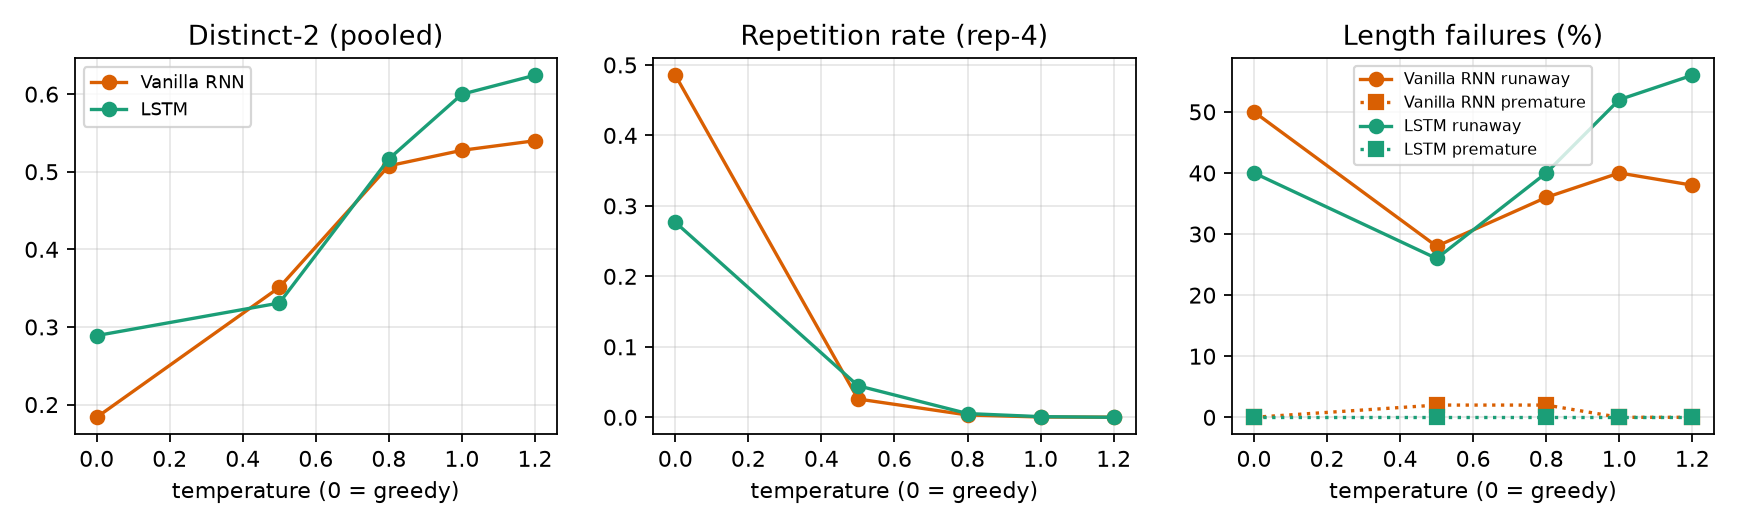
\includegraphics[width=\linewidth]{temperature_effect.png}
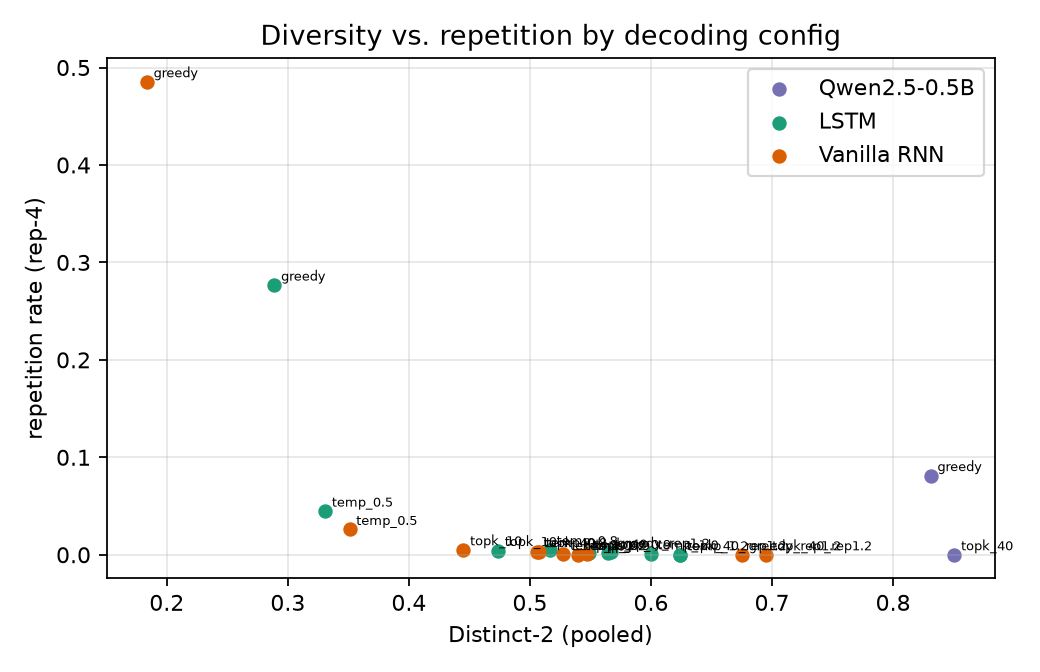
\includegraphics[width=0.62\linewidth]{diversity_vs_repetition.png}
\caption{Top: effect of temperature on diversity, repetition and length flags. Bottom: diversity
vs.\ repetition for every configuration.}\label{fig:temp}
\end{figure}

\begin{table}[H]\centering
\caption{Held-out termination test: the first sentence of each of 100 test stories is the prompt;
we generate up to 600 tokens (seed 0). Real = the remaining length of the actual story. Too long =
no \texttt{<eos>} or more than $2\times$ the real length.}\label{tab:length}
{\small\begin{tabular}{llrrrrrr}
\toprule
System & Config & Gen. mean & Gen. median & Real median & Premature\% & No \texttt{<eos>}\% & Too long\% \\
\midrule
Vanilla RNN & greedy & 461 & 600 & 176 & 0 & 73 & 73 \\
Vanilla RNN & temp\_0.8 & 174 & 110 & 176 & 0 & 0 & 16 \\
Vanilla RNN & topk\_40 & 162 & 167 & 176 & 0 & 0 & 3 \\
LSTM & greedy & 295 & 196 & 176 & 0 & 28 & 33 \\
LSTM & temp\_0.8 & 192 & 145 & 176 & 0 & 0 & 3 \\
LSTM & topk\_40 & 210 & 167 & 176 & 0 & 0 & 5 \\
\bottomrule
\end{tabular}
}
\end{table}

\section{The Plot-Twist Challenge (Part 4)}
\label{sec:twist}
We use the five openings from the brief. An examination paper already contains tomorrow's
answers. An old robot gets a message from its future version. A detective solves a murder
before it happens. A village cannot remember the previous day. A letter comes from 100 years
in the future. The exact wording is in \texttt{src/ptg/prompts.py}. Both models continued each
opening with all ten configurations and five seeds. We study greedy, temperature 0.8 and
top-$k$=40 in detail. We judge them on the four criteria of the brief: (1)~connection to the
prompt, (2)~a meaningful development or twist, (3)~consistency with earlier details, and (4)~no
excessive repetition or meaningless jumps.

\paragraph{The models cannot see several premises.} Any word outside the 7,590-word vocabulary
becomes \texttt{<unk>}. This affects these premise words: \emph{detective, murder, crime}
(detective prompt), \emph{examination, contained} (exam), \emph{version} (robot), \emph{previous}
(village) and \emph{addressed} (letter). So the models receive the detective prompt as ``the
\texttt{<unk>} solved the \texttt{<unk>} before the \texttt{<unk>} had even happened''.

\paragraph{Criteria judgements.} Table~\ref{tab:p4} scores the 30 RNN/LSTM continuations (seed 0;
greedy, $T=0.8$, top-$k$=40) and the 10 Qwen continuations. It uses the four criteria of the brief
(Yes = 1, Partial = 0.5, No = 0). Every judgement is in
\texttt{outputs/analysis/part4\_criteria.csv}, with a one-line reason. The analyst made these
judgements. The blinded LLM-judge ratings in Section~\ref{sec:eval} are a second, independent
check. Over all 60 judgements per model, the RNN got 0 Yes / 18 Partial / 42 No. The LSTM got
0 / 22 / 38.

\begin{table}[H]\centering
\caption{Plot-Twist criteria (mean over the 5 openings; Yes = 1, Partial = 0.5, No = 0).}\label{tab:p4}
{\small\begin{tabular}{llrrrr}
\toprule
System & Config & Connected & Twist & Consistent & No repetition \\
\midrule
Vanilla RNN & greedy & 0.00 & 0.00 & 0.20 & 0.20 \\
Vanilla RNN & temp\_0.8 & 0.10 & 0.00 & 0.30 & 0.40 \\
Vanilla RNN & topk\_40 & 0.00 & 0.10 & 0.20 & 0.30 \\
LSTM & greedy & 0.10 & 0.00 & 0.20 & 0.00 \\
LSTM & temp\_0.8 & 0.10 & 0.30 & 0.30 & 0.50 \\
LSTM & topk\_40 & 0.10 & 0.20 & 0.10 & 0.30 \\
Qwen2.5-0.5B & greedy & 1.00 & 0.50 & 0.90 & 0.90 \\
Qwen2.5-0.5B & topk\_40 & 0.90 & 0.60 & 0.70 & 1.00 \\
\bottomrule
\end{tabular}
}
\end{table}

\begin{enumerate}
\item \textbf{Connection to the prompt: almost none.} No RNN or LSTM continuation stays on the
  premise. The closest cases are weak echoes. The LSTM continues the village prompt with ``he forgot
  to remember its family''. It opens the letter prompt with ``excited to see what was inside''. It
  mentions ``a big machine'' after the robot prompt. An automatic check finds that 78\% (RNN) and
  62\% (LSTM) of Part~4 samples reuse no content word of the opening (Appendix~\ref{app:p4tab}).
\item \textbf{Twists are ready-made phrases.} When something surprising happens, it is a set phrase
  from TinyStories (``Suddenly, he heard a loud noise'', ``He couldn't believe his eyes'',
  ``It was a giant puppy!''). It never develops the premise. A few twists are truly strange. For
  example, the LSTM ends one continuation with ``the boat disappeared from the sky and the lake was all gone''.
\item \textbf{Consistency fails for characters.} The female student in the exam story becomes ``he''
  (Ex.~4). Sam becomes Tim, Joey, Jimmy, Joe and John within one passage. Characters thank
  themselves (``The dog was so happy and thanked the dog'').
\item \textbf{Repetition and jumps.} Greedy outputs repeat themselves in a loop (Ex.~1). Sampled
  outputs avoid repetition. But they jump between unrelated scenes (a monkey, a fisherman, a fish
  and a king in four sentences).
\end{enumerate}

\paragraph{The seed matters more than the prompt.} With the same seed and configuration, the RNN
gave the same 75-token continuation, word for word, for the detective and the village prompts
(Ex.~2 and~3). Table~\ref{tab:sens} shows that this is a general pattern. Take any sampling
configuration. Two continuations of \emph{different} prompts with the \emph{same} seed share more
4-grams than two continuations of the \emph{same} prompt with \emph{different} seeds. The gap is a
factor of 2--10. Up to 4--7\% of cross-prompt pairs start with the same 10 tokens. For cross-seed
pairs, this is 0\%. The recurrent state keeps so little of the opening that the random draw
decides the story.

\begin{table}[H]\centering
\caption{Prompt sensitivity (sampling configurations). Mean 4-gram Jaccard similarity between
continuations of different prompts with the same seed, and of the same prompt with different seeds.
Also, the share of cross-prompt pairs with identical first 10 tokens.}\label{tab:sens}
{\scriptsize\begin{tabular}{llrrr}
\toprule
System & Config & 4-gram Jaccard: diff. prompt, same seed & same prompt, diff. seed & Same first 10 tokens\% (diff. prompt) \\
\midrule
Vanilla RNN & temp\_0.5 & 0.025 & 0.016 & 0.889 \\
Vanilla RNN & temp\_0.8 & 0.034 & 0.004 & 4.444 \\
Vanilla RNN & temp\_1.0 & 0.044 & 0.001 & 1.778 \\
Vanilla RNN & temp\_1.2 & 0.084 & 0.000 & 2.667 \\
Vanilla RNN & topk\_10 & 0.015 & 0.004 & 0.444 \\
Vanilla RNN & topk\_40 & 0.022 & 0.001 & 0.000 \\
Vanilla RNN & topp\_0.9 & 0.048 & 0.001 & 4.000 \\
Vanilla RNN & topk\_40\_rep1.2 & 0.003 & 0.000 & 0.444 \\
LSTM & temp\_0.5 & 0.012 & 0.018 & 0.444 \\
LSTM & temp\_0.8 & 0.007 & 0.003 & 1.778 \\
LSTM & temp\_1.0 & 0.016 & 0.001 & 5.333 \\
LSTM & temp\_1.2 & 0.024 & 0.000 & 6.667 \\
LSTM & topk\_10 & 0.004 & 0.003 & 0.889 \\
LSTM & topk\_40 & 0.009 & 0.001 & 3.556 \\
LSTM & topp\_0.9 & 0.009 & 0.002 & 5.333 \\
LSTM & topk\_40\_rep1.2 & 0.006 & 0.001 & 2.667 \\
\bottomrule
\end{tabular}
}
\end{table}

\paragraph{RNN vs.\ LSTM in the challenge.} At $T=0.8$, the LSTM scores slightly higher on twist
and repetition (Table~\ref{tab:p4}). Its continuations drift less into stock characters
(12\% vs.\ 72\% at $T=0.8$ on the Part~4 prompts). It also keeps an unnamed ``he/she'' main
character for longer. The most important criterion is connection to the prompt. On this
criterion, the two models are equally poor.

\subsection*{Selected continuations (exact model output)}
\human{Ex.~1 illustrates: greedy repetition loop. Opening: Sam received a letter addressed to him from one hundred years in the future.}
\begin{modelout}{Ex. 1: Vanilla RNN, P4 letter, greedy, seed 0 (150 tokens, stop: max\_len)}
\small He wanted to play with it. He wanted to play with it. He wanted to play with the ball. He wanted to play with the ball. He wanted to play with the ball. He wanted to play with the ball. He wanted to play with the ball. He wanted to play with the ball. He wanted to play with the ball. He wanted to play with the ball. He wanted to play with the ball. He wanted to play with the ball. He wanted to play with the ball. He wanted to play with the ball. He wanted to play with the ball. He wanted to play with the ball. He wanted to play with the ball. He wanted to play with the ball. He wanted to play with the ball.
\end{modelout}

\human{Ex.~2 illustrates: prompt ignored (compare the next box). Opening: The detective solved the murder before the crime had even happened.}
\begin{modelout}{Ex. 2: Vanilla RNN, P4 detective, temp 0.8, seed 0 (75 tokens, stop: eos)}
\small Suddenly, he heard a loud noise. It made him feel sad and hurt. He tried to open the box, but he didn't know what to do. He swam back to the house and closed his eyes. He was happy when he put the flower in the water and it made bob feel better. He was so happy and thanked the magician for being a good helper.
\end{modelout}

\human{Ex.~3 illustrates: prompt ignored (same seed, different opening). Opening: One morning, the whole village woke up and discovered that nobody could remember the previous day.}
\begin{modelout}{Ex. 3: Vanilla RNN, P4 village, temp 0.8, seed 0 (75 tokens, stop: eos)}
\small Suddenly, he heard a loud noise. It made him feel sad and hurt. He tried to open the box, but he didn't know what to do. He swam back to the house and closed his eyes. He was happy when he put the flower in the water and it made bob feel better. He was so happy and thanked the magician for being a good helper.
\end{modelout}

\human{Ex.~4 illustrates: entity inconsistency: the student is female in the opening. Opening: A student opened her examination paper and saw that it already contained the answers to tomorrow's questions.}
\begin{modelout}{Ex. 4: LSTM, P4 exam, temp 0.8, seed 0 (150 tokens, stop: max\_len)}
\small Suddenly, he heard a loud noise and looked out the window. He saw a big, colorful balloon. It was shiny! It croaked from the ceiling and heard a loud noise. It was a loud noise and he looked around. He couldn't believe his eyes and it started to move in the sky. He was very surprised and so he ran towards it. The little boy was so excited and he ran to the playground. He jumped up in the air and the old bear started to blow. He just couldn't believe it forever. The boy was so excited! He hugged the bear and waved goodbye as the man was happy to have his home. He woke up with a small smile and watched the sun go down, and it was time to go
\end{modelout}

\human{Ex.~5 illustrates: high temperature. Opening: The detective entered the abandoned house and noticed that every clock had stopped at exactly midnight. Suddenly, the telephone rang...}
\begin{modelout}{Ex. 5: LSTM, P3 mystery, temp 1.2, seed 0 (150 tokens, stop: max\_len)}
\small Popcorn lay down and started his vacation back. Between the sunshine, all one answered, who demanded that the storm touched; spring was fragile, but then something heard the noise quickly. It was a loud noise outside from wide, smaller light! Molly couldn't believe what she had excitedly. She wanted her mother in warning. And nothing out, then something happened. How curl the pose may find something useful, there was all bright and white! Mama asked: "mommy, can that my avocados would happen in the sunny place where it go?". Mama nodded its head, keeping mike mad and enjoy the patient before she was only waiting at it. Emma woke up with her mom and felt very old. She started wearing more and more others all over
\end{modelout}

\human{Ex.~6 illustrates: repetition penalty on greedy decoding. Opening: The detective entered the abandoned house and noticed that every clock had stopped at exactly midnight. Suddenly, the telephone rang...}
\begin{modelout}{Ex. 6: Vanilla RNN, P3 mystery, greedy rep1.2, seed 0 (132 tokens, stop: eos)}
\small It was a big, scary monster! The bird was very sad because he wanted to go on an adventure. So, he decided to take a nap in his pocket. But then, something bad happened. The little boy saw a big tree with lots of leaves. Timmy loved to play with his toys all day long. One day, tim's mom asked him to help her find a new toy. Lily said yes and they went to the store. She found some yummy snacks and put them in a bowl. "Look, mommy! I'm going to get my ball!" she exclaimed. "You're welcome, lily. You are very kind."
\end{modelout}

\human{Ex.~7 illustrates: zero-shot LLM baseline. Opening: An old robot lived alone in a quiet shed. One morning, it received a message from its future version.}
\begin{modelout}{Ex. 7: Qwen2.5-0.5B, P4 robot, topk 40, seed 0 (44 tokens, stop: eos)}
\small After much contemplation, the old robot decided to play along. It received a message from its future self warning of an approaching threat, but instead of rushing out, it decided to take a moment to reflect on the situation.
\end{modelout}


\section{Is the better language model also the better storyteller? (Part 5)}
\label{sec:eval}
\subsection{Quantitative evaluation}
Table~\ref{tab:quant} shows the results of the two trained models. Both use the same held-out test
split and the same generation grid: 10 prompts $\times$ 10 configurations $\times$ up to 5 seeds =
420 continuations per model. The settings are in \texttt{outputs/generations/generation\_settings.json}.

\begin{table}[H]\centering\small
\caption{Quantitative comparison (all configurations pooled together). Per-sample Distinct is the
mean over samples. Pooled Distinct counts unique $n$-grams over all 420 samples.}\label{tab:quant}
\begin{tabular}{lrr}
\toprule
 & Vanilla RNN & LSTM \\
\midrule
Validation / test perplexity & 16.00 / 15.77 & \textbf{11.99 / 11.81} \\
Distinct-1 / Distinct-2 (pooled) & 0.045 / 0.267 & 0.043 / 0.279 \\
Distinct-1 / Distinct-2 (per-sample mean) & 0.698 / 0.946 & 0.630 / 0.924 \\
Repetition rate (Rep-4) / loops & 0.016 / 1.4\% & 0.014 / 1.0\% \\
Mean generated length (tokens) & 103.8 & 130.4 \\
Premature (\texttt{<eos>} $<$20 tokens) & 1.4\% & 0.0\% \\
Reached 150-token limit & 36.9\% & 45.2\% \\
Held-out test, greedy: no \texttt{<eos>} in 600 tokens & 73\% & 28\% \\
Off-prompt / stock character & 67.6\% / 71.4\% & 49.8\% / 33.1\% \\
\bottomrule
\end{tabular}
\end{table}

The RNN has \emph{higher} per-sample Distinct values. This is partly an effect of length. Its
continuations are shorter (104 vs.\ 130 tokens), and Distinct-$n$ falls as texts get longer. When
we compare the same configuration at $T\geq1.0$, the LSTM's pooled Distinct-2 is higher
(0.60--0.62 vs.\ 0.53--0.54).

\subsection{Blinded evaluation (LLM judges as a proxy for human raters)}
\paragraph{Design.} We fixed the sample set in the configuration file before we read any output.
It covers every Plot-Twist opening $\times$ \{Vanilla RNN, LSTM, Qwen\} $\times$ \{temperature 0.8,
top-$k$=40\}, with seed 0. This gives 25 samples (the LLM uses top-$k$=40 only). The surface form
of the text should not reveal the system. So every system's output goes through the same word
tokenizer, lowercasing, detokeniser and 150-token cap. We shuffled the samples (seed 2026) and gave
them anonymous IDs. We showed each sample with its opening on an HTML sheet. The key (which ID
belongs to which system) was kept in a separate file. Each rater rated every sample on their own,
from 1 to 5. The criteria were coherence, grammatical quality, relevance to the opening, and
creativity/surprise. We measure agreement with Krippendorff's $\alpha$ (ordinal). We compare LSTM
and RNN with a paired Wilcoxon signed-rank test over the 10 (opening, config) pairs. For each pair
we use the mean over raters.

\paragraph{Raters: LLM judges, not people.} The brief asks for at least three human evaluators
``wherever feasible''. We could not run a human study before our deadline. So the ratings come from
three LLM judges: Claude Haiku~5.5, Claude Sonnet~5.5 and Claude Opus~5.5 (Anthropic). Each judge
ran as a separate agent. Each judge got only the blinded sheet (\texttt{sheet.csv}: ID, opening,
continuation) and the instructions written for human raters. We told each judge not to open any
other project file. Each judge wrote one CSV (\texttt{outputs/human\_eval/ratings/llm\_judge\_*.csv}),
which we kept unedited. \textbf{These scores are a proxy for human judgement, not a replacement for
it.} There are three caveats: (i)~LLM judges tend to prefer fluent, well-formed text, and this helps
the LLM baseline; (ii)~the three judges come from one model family and may share biases, so their
agreement is likely higher than that of independent people; (iii)~their scores have not been checked
against human ratings on this data. The sheet and template are ready for a human study
(\texttt{outputs/human\_eval/README.md}).

\paragraph{Results.} The three judges rated all 25 samples (300 ratings; Table~\ref{tab:human},
Fig.~\ref{fig:human}).
\begin{itemize}
\item \textbf{RNN and LSTM get the same ratings, close to the lowest score.} Coherence 1.40 vs.\ 1.37,
  relevance 1.10 vs.\ 1.17, creativity 1.00 vs.\ 1.13 (RNN vs.\ LSTM). Grammar gets higher ratings
  (about 2.7) but is still poor. No LSTM--RNN difference is significant (paired Wilcoxon over the 10
  opening$\times$config pairs, $p\geq0.25$ for every criterion; Table~\ref{tab:lstmrnn}).
\item \textbf{The LLM gets much higher ratings} on grammar (4.67), relevance (4.13) and coherence
  (3.87). But it gets only 2.40 on creativity. The judges' comments match our own observation. The
  LLM stays on topic, but it turns the twist into a moral or drops the paradox (S21, S22).
\item \textbf{Agreement} is substantial (Krippendorff's $\alpha$ 0.66--0.76; Table~\ref{tab:agree}).
  But two things make it look higher than it really is. One is the large gap between the LLM and the
  trained models. The other is a floor effect: RNN creativity is 1 in all 30 ratings, so there is
  little room to disagree. No sample's ratings differ by more than 2 points. The two samples with the
  most disagreement are these. S05 is Qwen on the village opening (relevance 2--4): it keeps
  the village but ignores the memory loss. S04 is the RNN on the detective opening (grammar 3--5): it
  gives two clean sentences unrelated to the opening.
\item \textbf{Automatic metrics vs.\ ratings} (Spearman over the 25 samples; Table~\ref{tab:corr}).
  Prompt overlap rises together with relevance ($\rho=0.69$, $p<0.001$) and creativity ($\rho=0.51$,
  $p=0.01$). This supports its use as a relevance proxy. Distinct-2 is unrelated to every criterion
  ($|\rho|\leq0.18$, $p\geq0.39$). Longer continuations get lower ratings for coherence and grammar
  ($\rho=-0.58$, $p=0.002$). This is mostly because the LLM writes shorter and better text. So length
  and system are confounded: we cannot separate their effects.
\end{itemize}

\begin{table}[H]\centering\caption{Blinded ratings by three LLM judges (1--5, mean $\pm$ sd over all
ratings; 15 ratings for Qwen, 30 for each trained model).}\label{tab:human}
\begin{tabular}{lllll}
\toprule
System & Coherence & Grammar & Relevance & Creativity \\
\midrule
Qwen2.5-0.5B-Instruct & 3.87 $\pm$ 0.52 & 4.67 $\pm$ 0.62 & 4.13 $\pm$ 0.99 & 2.40 $\pm$ 1.12 \\
LSTM & 1.37 $\pm$ 0.49 & 2.67 $\pm$ 0.61 & 1.17 $\pm$ 0.38 & 1.13 $\pm$ 0.35 \\
Vanilla RNN & 1.40 $\pm$ 0.50 & 2.73 $\pm$ 0.87 & 1.10 $\pm$ 0.31 & 1.00 $\pm$ 0.00 \\
\bottomrule
\end{tabular}
\end{table}
\begin{table}[H]\centering\caption{Agreement between the three LLM judges.}\label{tab:agree}
\begin{tabular}{lrr}
\toprule
Criterion & Krippendorff's alpha (ordinal) & Mean within-sample sd \\
\midrule
coherence & 0.73 & 0.28 \\
grammar & 0.70 & 0.41 \\
relevance & 0.76 & 0.22 \\
creativity & 0.66 & 0.18 \\
\bottomrule
\end{tabular}
\end{table}
\begin{table}[H]\centering\caption{LSTM vs.\ Vanilla RNN: mean judge rating over the 10
(opening, config) pairs and paired Wilcoxon signed-rank test.}\label{tab:lstmrnn}
\begin{tabular}{lrrrr}
\toprule
Criterion & Pairs & LSTM mean & RNN mean & Wilcoxon $p$ \\
\midrule
coherence & 10 & 1.367 & 1.400 & 1.000 \\
grammar & 10 & 2.667 & 2.733 & 0.824 \\
relevance & 10 & 1.167 & 1.100 & 0.500 \\
creativity & 10 & 1.133 & 1.000 & 0.250 \\
\bottomrule
\end{tabular}
\end{table}
\begin{table}[H]\centering\caption{Spearman $\rho$ between automatic metrics and the mean judge
rating of each sample (25 samples).}\label{tab:corr}
\begin{tabular}{lrrrr}
\toprule
 & Coherence & Grammar & Relevance & Creativity \\
\midrule
Distinct-2 & 0.13 & 0.05 & -0.06 & -0.18 \\
Length & -0.58 & -0.58 & -0.22 & 0.01 \\
Prompt overlap & 0.20 & 0.12 & 0.69 & 0.51 \\
Rep-4 & -0.19 & -0.20 & -0.28 & 0.05 \\
\bottomrule
\end{tabular}
\end{table}
\begin{figure}[H]\centering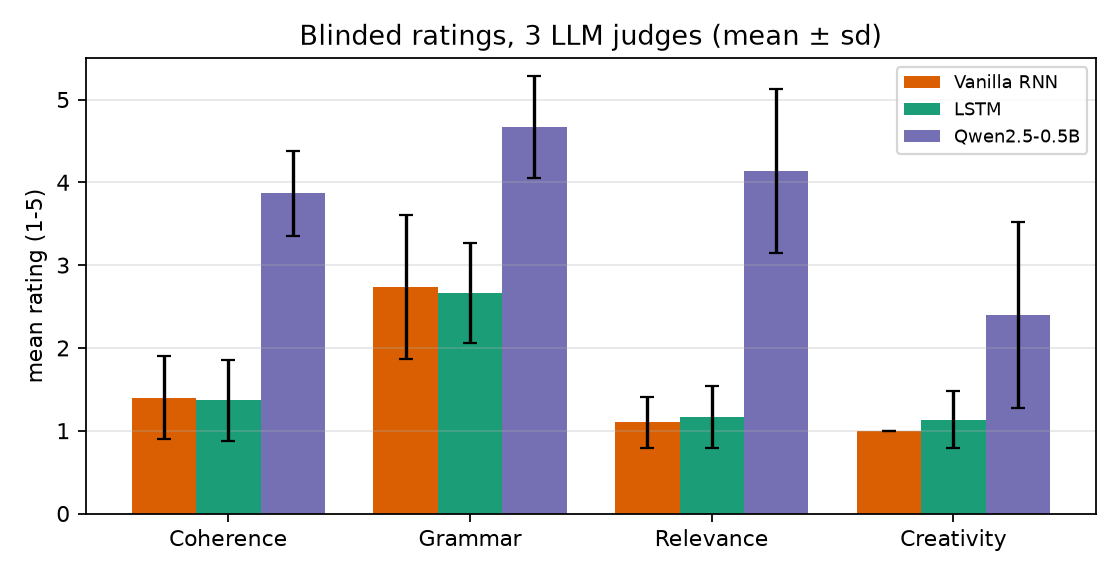
\includegraphics[width=0.75\linewidth]{human_eval.png}
\caption{Blinded LLM-judge ratings per system (mean $\pm$ sd).}\label{fig:human}\end{figure}

\section{Optional extension: a zero-shot open-source LLM}
\label{sec:llm}
\textbf{Checkpoint}: \texttt{Qwen/Qwen2.5-0.5B-Instruct} in \textbf{fp16}, on the same GPU, \textbf{not fine-tuned}.
Its exact revision is recorded in \texttt{outputs/generations/llm\_settings.json}.
\textbf{Prompt template} (chat format, built with the tokenizer's chat template): system ``You are a
storyteller who writes short, simple stories for children.''; user ``Continue this story. Write the
next part in simple English (about 120 words). Write only the continuation. Story opening:
\{opening\}''. \textbf{Decoding}: greedy and top-$k$=40 ($T$=1, top-$p$=1, repetition penalty 1.0).
We set these values explicitly so that the checkpoint's own defaults do not apply. We use 5 seeds
and at most 220 subword tokens. We then re-tokenise the output with our word tokenizer and cut it
to 150 tokens, as for the RNN and LSTM. We do not compare perplexity, because the tokenizers differ.

\paragraph{Results.} The LLM is far better at staying connected to the prompt. It reuses 32--41\%
of the opening's content words (RNN/LSTM: 0--10\%). Only 7\% of its samples are off-prompt. Its
Part~4 criteria scores are 0.9--1.0 for connection and 0.7--0.9 for consistency
(Table~\ref{tab:p4}). But it is not a good storyteller either. It tends to explain the twist away
(the exam student ``was about to take it''). It may instead turn the twist into a moral (``the
importance of thorough preparation''; Ex.~7 is one of its better outputs). Or it ignores the
paradox (the detective's case has ``the victim's family'' and a crime scene, although the crime has
not happened). It also contradicts itself. ``Mr.\ Green'' is the village elder and then turns to
``the village elder''. A letter from 100 years ahead arrives ``after centuries''. Its continuations
are shorter: 77 tokens on average, and 8\% end within 20 tokens with top-$k$=40. Its greedy output
repeats a whole sentence word for word. Its higher Distinct values come partly from its
shorter texts and smaller sample (30 vs.\ 420). So they are not directly comparable. The common failure types differ. The RNN and LSTM fail by \emph{forgetting the prompt}.
The LLM fails by \emph{under-using} it: it gives a safe, literal reading instead of a twist.

\section{Final analysis (Part 6)}
\label{sec:analysis}
\paragraph{Q1. How do the Vanilla RNN and LSTM differ in modelling sequential text?} The LSTM
models TinyStories much better. Its test perplexity is 11.81 vs.\ 15.77, with the same width and
training budget. Three observations suggest that the reason is \emph{longer memory}, not just more
parameters. (i)~Its advantage is very small on the first 8 tokens (0.04 nats). It is stable at
about 0.31 nats once 32 or more tokens of context are available (Fig.~\ref{fig:grad}). (ii)~The
RNN's gradients spike up to $39\times$ the clipping threshold. The LSTM's gradients stay below
1.62. Gating keeps the gradient flow stable over long sequences. The tanh RNN's gradient flow is
not stable. (iii)~The RNN learns faster at first but levels off earlier (Fig.~\ref{fig:loss}).
One caveat: the LSTM has 1.4$\times$ the parameters (9.51M vs.\ 6.76M; 4$\times$ the recurrent
weights). We did not train an RNN with a matched number of parameters. So part of the gap may come
from capacity (model size). However, the gap changes with token position, and capacity alone
cannot easily explain this.

\paragraph{Q2. Which model generates more coherent and less repetitive continuations?} The LSTM,
on every automatic measure:
\begin{itemize}
\item fewer greedy loops (40\% vs.\ 60\%; Rep-4 0.28 vs.\ 0.49);
\item far fewer greedy runs that never stop, on held-out stories (28\% vs.\ 73\%);
\item better-calibrated lengths;
\item fewer jumps to stock characters (33\% vs.\ 71\%) and fewer off-prompt samples (50\% vs.\ 68\%).
\end{itemize}
In the analyst's judgements, it scores slightly higher on twist and repetition. For
\emph{coherence}, the difference is only a matter of degree. Both models write sentences that are
grammatical locally but do not form a plot. The blinded LLM judges see no difference. Coherence is
1.37 (LSTM) vs.\ 1.40 (RNN), and grammar is 2.67 vs.\ 2.73 (Wilcoxon $p=1.0$ and $0.82$). The
rated samples use $T=0.8$ and top-$k$=40. With these settings, neither model loops (0\% loop rate
for both). The LSTM's advantage is in greedy decoding and in ending stories. The rated set does not
cover these. So the LSTM is less repetitive, but neither model is coherent to a reader.

\paragraph{Q3. How does temperature affect creativity and grammatical quality?} It pushes them in
opposite directions, and monotonically (the trend never reverses). As $T$ rises from 0.5 to 1.2,
Distinct-2 rises from 0.33--0.35 to 0.54--0.62. Rep-4 falls to zero. Above $T\approx1.0$, grammar
gets visibly worse (Ex.~5) and the share of LSTM samples that jump to a stock character rises from
12\% to 58\%. Low temperatures give safe, repetitive, generic text. High temperatures give novelty,
but it is random rather than creative. A new word is not a new plot development. $T=0.8$ or
top-$k$=40 gives the best balance for these models.

\paragraph{Q4. Can higher diversity scores guarantee better stories?} No. Among the trained models,
the settings with the highest Distinct-2 are top-$k$+penalty (0.70), greedy+penalty for the RNN
(0.68) and $T=1.2$. These are among the least coherent. For the RNN, 70--100\% of their samples are
off-prompt. Characters keep changing, and grammar breaks at $T=1.2$. The RNN even has a higher
per-sample Distinct than the LSTM, although it is worse on every other measure. Diversity is
\emph{necessary} to avoid loops: greedy is both the least diverse and the most broken. But
diversity is not enough on its own. Distinct-$n$ rewards novelty whether or not it makes sense. It
is also sensitive to length.
The blinded ratings confirm this. Distinct-2 has no relation to the judges' scores for creativity
($\rho=-0.18$, $p=0.39$) or coherence ($\rho=0.13$, $p=0.53$). Prompt overlap does relate to them
(creativity $\rho=0.51$, relevance $\rho=0.69$; Table~\ref{tab:corr}).

\paragraph{Q5. Does lower perplexity correspond to better storytelling?} Only partly. The LSTM's
lower perplexity shows up as better \emph{local} behaviour: fewer loops, better length calibration
and fewer character switches. It does not show up as better \emph{storytelling}. Both models
ignore the premise of the opening. They produce stock twists, not meaningful ones. With the same
seed, they generate almost the same text for different prompts. Perplexity measures how well a
model predicts typical TinyStories text one token at a time. Our prompts are unusual on purpose
(detectives, exams, time travel), and some of their words are out of vocabulary. A good
continuation must be conditioned on that prompt. It also needs world knowledge and plot planning.
Next-token perplexity rewards none of these. The blinded ratings agree. The LSTM's 25\% lower
perplexity brings no measurable gain with the judges. On the 1--5 scale, LSTM minus RNN is $-0.03$
(coherence), $-0.07$ (grammar), $+0.07$ (relevance) and $+0.13$ (creativity). None is significant
($p\geq0.25$). Both models stay below 3 on every criterion. We cannot
compare perplexity with the LLM. But the LLM's text is far more fluent and on-topic, and it is
rated much higher (coherence 3.87). Even so, it gets only 2.40 on creativity. These are LLM-judge
ratings, not human ones (Section~\ref{sec:eval}).

\paragraph{Q6. Most frequent failures and how to reduce them.} From most to least frequent
(Tables~\ref{tab:fail}, \ref{tab:p4}):
\begin{enumerate}
\item \emph{Prompt forgetting / off-prompt drift} (50--68\% of samples; 62--78\% on the Part~4
  openings) $\rightarrow$ subword tokenisation, so that prompt words are never \texttt{<unk>}; more
  training data, with more variety; an attention mechanism (or Transformer), so that the model can
  still look back at the prompt; prompts closer to the training domain.
\item \emph{Falling back to stock characters and plots} (33--71\%) $\rightarrow$ a larger and more
  varied corpus; moderate temperatures ($T\leq0.8$) for the LSTM.
\item \emph{Inconsistent entities} (gender, names; most Part~4 samples) $\rightarrow$ architectures
  with longer memory; decoding that keeps track of entities, or constraints.
\item \emph{Repetition loops and stories that never stop, with greedy decoding} (40--73\%)
  $\rightarrow$ sampling, top-$k$/top-$p$, a repetition penalty or $n$-gram blocking. All of these
  remove the loops in our runs. The penalty must be mild, because it also makes characters keep
  changing.
\item \emph{Ungrammatical output at high temperature} $\rightarrow$ top-$k$/top-$p$ truncation and
  $T\approx0.8$.
\end{enumerate}

\paragraph{Q7. Limitations of a small LM trained on a limited corpus.} (i)~\emph{Data}: 20k stories
(4.2M tokens) of children's English that is simple on purpose. The vocabulary of 7,590 words is
missing basic words from the twist prompts. The stories also teach a narrow set of plots and
characters, and the models fall back on them. (ii)~\emph{Architecture}: a fixed-size recurrent
state must hold a compressed form of the whole prompt. Without attention, most of the opening is
lost after a few sentences (Table~\ref{tab:sens}). (iii)~\emph{Training}: we used one seed per
model and a 15-epoch budget. Neither model had converged by then. (iv)~\emph{Evaluation}:
automatic metrics measure repetition and diversity but not plot. Our Part~4 judgements come from
one analyst. The blinded ratings come from LLM judges, not from people. The rated set is small
(25 samples). Even with identical formatting, it cannot fully hide the LLM's fluency. We cannot
compare perplexity with the LLM because the tokenisers differ. Even so, the qualitative picture
(fluent sentences, no story) was the same for every prompt, seed and configuration we looked at.

\section{Reproducibility}
All hyper-parameters are in \texttt{configs/default.yaml}. Seeds: 42 (split, initialisation,
batching) and 0--4 (generation). For every run, we save the resolved configuration, command-line
arguments and hardware in \texttt{outputs/configs\_used/}. A log with timestamps is in
\texttt{outputs/run\_log.txt}. The command \texttt{python -m ptg.cli all} reproduces every number
and figure. cuDNN RNN kernels are not bit-for-bit deterministic. So retraining may change the last
decimals. The submitted checkpoints reproduce the reported numbers.
\appendix
\section{Next-token training pairs}\label{app:pairs}
\begin{small}
\verbatiminput{tables/input_target_pairs.txt}
\end{small}

\section{Part 3 examples (verbatim, seed 0)}\label{app:p3}
Two of the five Part~3 prompts under six configurations; all others are in
\texttt{outputs/stories/part3\_stories.md}.
\subsubsection*{P3 mystery (a mystery)}
\human{Opening (human-written): The detective entered the abandoned house and noticed that every clock had stopped at exactly midnight. Suddenly, the telephone rang...}

\begin{modelout}{Vanilla RNN, greedy, seed 0 (85 tokens, stop: eos)}
\small The bird was very sad and scared. The bird was scared and didn't know what to do. He tried to get the ball, but he couldn't find it. He tried to get the ball, but it was too late. He was so sad and he couldn't wait to play with his friends. He was so happy and thanked the man. He thanked the man and said, "thank you, mommy!"
\end{modelout}

\begin{modelout}{Vanilla RNN, temp 0.5, seed 0 (39 tokens, stop: eos)}
\small The frog was gone. His mom told him that it was not important to share his toys and not to worry. He said he could have a new friend and he was very proud of him.
\end{modelout}

\begin{modelout}{Vanilla RNN, temp 0.8, seed 0 (74 tokens, stop: eos)}
\small Then he saw the way back in the water. The fox was so proud of himself and he started to cry. He knew he had to do it to tell his mom quickly. They both put the ball on the wide plane and turned the water back. They were so happy! From bob was on the other side, he felt so happy and content. The end.
\end{modelout}

\begin{modelout}{Vanilla RNN, temp 1.2, seed 0 (150 tokens, stop: max\_len)}
\small Then he saw the way his ball back. He knew that being persistent meant and brought true foods's room. No one knew it croaked, but then something heard happened. Bobo was very happy! He thanked the bug and missed the ball after friends. "Goodbye for happiness safety!" bob was so excited that he forgot and sang so much fun! Eventually, the skeleton johnny pose and keeping playing with their bucket. Jay went to the bathroom, and he thanked the old bear that was filled a lot of fun sunny of the interesting apples. He sang up and then soaring over the stairs. Dotty was upset again before taking his pan with his friends. Acorns woke up with her small sack and licks the boat tightly. After they finished, she hugged back
\end{modelout}

\begin{modelout}{Vanilla RNN, topk 40, seed 0 (150 tokens, stop: max\_len)}
\small Then he saw the mess. It was a funny dog. It was friendly and shiny and he wanted to catch a tree! It broke from the ceiling and broke it with a hat. It was loud and scary. Lily was sad and angry. She said, "sorry, lily. She did not mean to hurt. And I'm sorry for you. I told you to listen to her and be careful. You are a big knight." sara and ben nod. She hugs him. "You helped me stay away from the fountain." tom says. They sit on the grass and go outside. The car goes and goes on the floor. It is hard to make a mess! They cannot reach the top, behind a big puddle. It
\end{modelout}

\begin{modelout}{Vanilla RNN, topk 40 rep1.2, seed 0 (150 tokens, stop: max\_len)}
\small Then he saw the mess his ball back when he came out of him. Then, a kind fox named sammy went to the store to play with it. Lily was curious but timmy didn't know what you needed. Timmy was sad because he could not reach the bird or the park. Bob wanted to make something special. Later that day, jimmy's owner took him home outside to get her passport. They both got angry and threw it into a spot. He gave them carefully to him some tools for jack. "Where did it go away?" timmy nodded eagerly. He looked around and saw lots of people, so one morning came at tim. He couldn't figure any new friends! All the kids were amazed, they knew how many fun things
\end{modelout}

\begin{modelout}{LSTM, greedy, seed 0 (130 tokens, stop: eos)}
\small It was a big, scary monster. The bear was scared and he ran away. The bear was scared and he wanted to help. He ran to the door and saw the bear. He was so excited! He ran to the door and saw a big, scary bear. The bear was scared and ran away. The bear was scared and he ran away. The bear was very sad. He wanted to help the rabbit. He asked his mom if he could go to the hospital. The doctor said yes, but the rabbit was too scared. He was very sad. He was very sad. He wished he had been able to help the rabbit.
\end{modelout}

\begin{modelout}{LSTM, temp 0.5, seed 0 (137 tokens, stop: eos)}
\small It was a big, scary monster! The crocodile was very scared and he ran away. He was scared and scared. He wanted to be brave and explore the world. But then, something strange happened. The hunter looked around and saw a big, old man. He had never seen anything like it before. He was so scared that he ran towards the old man. The man looked around and saw a big, black dog. He was so scared that he started to cry. The boy was scared and he ran away. The man was very sad. He wished he had been brave and wanted to stay away. The little boy was happy and he knew he had to be careful.
\end{modelout}

\begin{modelout}{LSTM, temp 0.8, seed 0 (150 tokens, stop: max\_len)}
\small It was a big, weak monster! The crocodile was very scared and hurt. He tried to open the box but he was too fast. He dropped the jet and jumped quickly. He was scared, but he didn't want to leave the big tree. He cried and shook his head against his nose. But then, he heard a voice. The kitten said, "I don't know, I'm sorry. I won't hurt you." the monkey was sad, but he was a bit fearful. He was very sad and wanted to go to the store. He reached out and caught out of the bird. The cat was scared and ran away from the mouse. The bear felt very lucky. He had been sick and he was glad to
\end{modelout}

\begin{modelout}{LSTM, temp 1.2, seed 0 (150 tokens, stop: max\_len)}
\small Popcorn lay down and started his vacation back. Between the sunshine, all one answered, who demanded that the storm touched; spring was fragile, but then something heard the noise quickly. It was a loud noise outside from wide, smaller light! Molly couldn't believe what she had excitedly. She wanted her mother in warning. And nothing out, then something happened. How curl the pose may find something useful, there was all bright and white! Mama asked: "mommy, can that my avocados would happen in the sunny place where it go?". Mama nodded its head, keeping mike mad and enjoy the patient before she was only waiting at it. Emma woke up with her mom and felt very old. She started wearing more and more others all over
\end{modelout}

\begin{modelout}{LSTM, topk 40, seed 0 (150 tokens, stop: max\_len)}
\small It was a big, strong monster! Mama went to pick up the puppy and brought it to the door. A giant man appeared in a big bag. He said, "please, I will help you get your money in the cage!" the old man took off the hat and ran away. Mommy was sad. Then the old man's daughter heard a voice: "don't worry, I'll help you. I will have some cake and food." mummy carefully said, "a piece of my clothes will help them go." he smiled and wiped the big bite off his hands. When the man was ready out of his work, he gave his mom some delicious cream and a surprise. Mommy said, "it was a fun day
\end{modelout}

\begin{modelout}{LSTM, topk 40 rep1.2, seed 0 (150 tokens, stop: max\_len)}
\small It was a big, strong monster! Mama went to pick up her puppy and brought him some of the vegetables in the oven. She tried to copy the answer but then it was time for him to reach again. But he didn't want to be sad and cried. The little penguin ran away and tried to get back home. So, he started eating a big smile instead of noise. Finally, they found a few white spot outside from a nearby tree. The old bear said, "look what you have done talking and it is very important." henry saw the spider's tail and wanted to catch the bird better and he kept its eye. He soon pulled out some small pieces and put the net in his bag. His mom smiled as she
\end{modelout}







\subsubsection*{P3 discovery (a surprising discovery)}
\human{Opening (human-written): While digging in the garden, Ben found an old wooden box. When he opened it, he could not believe his eyes.}

\begin{modelout}{Vanilla RNN, greedy, seed 0 (150 tokens, stop: max\_len)}
\small He was so excited! He ran to the edge of the hill and saw a big, scary dog. He was so excited! He ran to the edge of the hill and saw a big, scary dog. He was so excited! He ran to the edge of the hill and saw a big, scary dog. He was so excited! He ran to the edge of the hill and saw a big, scary dog. He was so excited! He ran to the edge of the hill and saw a big, scary dog. He was so excited! He ran to the edge of the hill and saw a big, scary dog. He was so excited! He ran to the edge of the hill and saw a big, scary dog. He was so
\end{modelout}

\begin{modelout}{Vanilla RNN, temp 0.5, seed 0 (75 tokens, stop: eos)}
\small He was so happy. His mommy said, "you're welcome, timmy. You are my best friend." the boy smiled and said, "I will help you." the little boy smiled and said, "thank you, lily. You are so smart and brave!" bob was so happy that he forgot to be so good for the rest of the day.
\end{modelout}

\begin{modelout}{Vanilla RNN, temp 0.8, seed 0 (75 tokens, stop: eos)}
\small Suddenly, he heard a loud noise. It made him feel sad and hurt. He tried to open the box, but he didn't know what to do. He swam back to the house and closed his eyes. He was happy when he put the flower in the water and it made bob feel better. He was so happy and thanked the magician for being a good helper.
\end{modelout}

\begin{modelout}{Vanilla RNN, temp 1.2, seed 0 (102 tokens, stop: eos)}
\small Suddenly he saw the way his ball and gave him a big man's mechanic. Paw felt sad that he knew no one want to go now. Then, he sat down quickly fell asleep. Everything could reach again! Wide missed the ball after a few seconds and johny off safety! From bob he was much hero warning. And the ball was very tall. Daddy told the present to always find something useful for help before eating games. He shared them; he was so happy that that was was a great time!
\end{modelout}

\begin{modelout}{Vanilla RNN, topk 40, seed 0 (77 tokens, stop: eos)}
\small Suddenly he saw the mess. It was a funny dog. It was friendly and shiny and he wanted to catch a tree! He picked it up and carried it to his friends. They both put the flag on the paper, and the door was delicious. They were so happy! From bob was on the other side, and the old man's friends were happy with the work together.
\end{modelout}

\begin{modelout}{Vanilla RNN, topk 40 rep1.2, seed 0 (25 tokens, stop: eos)}
\small Suddenly he saw a big tree in the middle of the lake. He asked his mom if they could keep it from him!
\end{modelout}

\begin{modelout}{LSTM, greedy, seed 0 (75 tokens, stop: eos)}
\small He was so excited! He ran to the kitchen and saw a big, round ball. He wanted to play with it. He ran to the slide and started to climb. He was so happy. He ran around the park and laughed. He was so happy. He had a great time. He was so happy. He had a great time playing with his new toy.
\end{modelout}

\begin{modelout}{LSTM, temp 0.5, seed 0 (112 tokens, stop: eos)}
\small He was so excited. His mom said, "let's make it go." so, they went to the kitchen. It was a big, juicy rock. They were so excited. They played with the ball and laughed. When the sun was over, they went to the park. They saw a big tree. It was so high and tall. The sun was shining and it was very hot. It was so bright and pretty. Ben and his mom were very happy. They played together for a while, but then it was time to go home.
\end{modelout}

\begin{modelout}{LSTM, temp 0.8, seed 0 (143 tokens, stop: eos)}
\small He was so excited. His mommy told him he needed to make it more treasures, so he took the diary home. Bob's mom tried to move the jet away, but it was too late. It was not wide, but it couldn't break. John cried and shook his head. He was scared that he could get very upset. Then, an old man came outside to get a big box. He told his mom what he had seen; he was so old. The old man smiled and said he must be a little girl. He was so mad! The man was very upset and missed the man before taking his pan. He was so happy to see his new sister and have a lot of fun.
\end{modelout}

\begin{modelout}{LSTM, temp 1.2, seed 0 (88 tokens, stop: eos)}
\small Ben lay down and started his adventure. When he came back, he put his paw on the grass. It touched the ground and croaked, but then something heard him move quickly. It was a loud noise outside from wide, smaller light! He couldn't believe what it had! From bob was almost startled in warning. And nothing seemed really scary! Eventually, zip giggled and pose it silent. He was so thankful to be with it!
\end{modelout}

\begin{modelout}{LSTM, topk 40, seed 0 (150 tokens, stop: max\_len)}
\small He was so happy. His mommy told him he needed to make him feel better, so he took the box from the ground and took a bite. As he sat, his mum appeared and said, "good job, mommy! Can you please help me and give it to me?" he was amazed by how he could read out how he ate. His mom said, "it's easy to be patient and don't lose it!" he was so excited. She said, "I will help you find the way back home." he smiled and wiped the big water off his hands. When the sun was ready, he gave it a special pat to make with his family and all the treats. They went to his garden and enjoyed the
\end{modelout}

\begin{modelout}{LSTM, topk 40 rep1.2, seed 0 (71 tokens, stop: eos)}
\small Suddenly he saw a big pile of colorful water in the sunshine. He put his hands on the grass and put them underneath the ground. Now, it was a magical place for ben's house! After a bath, john was able to stay down through the forest for an adventure! From then on, they jogged in their home and had lots of fun.
\end{modelout}








\section{Part 4 metrics and examples (verbatim, seed 0)}\label{app:p4tab}
\begin{table}[H]\centering
\caption{Automatic metrics on the five Plot-Twist openings only.}
{\scriptsize\resizebox{\linewidth}{!}{\begin{tabular}{llrrrrrrrr}
\toprule
System & Config & D-1 & D-2 & Rep-4 & Sent.rep & Len & Prem.\% & Runaway\% & Overlap \\
\midrule
Vanilla RNN & greedy & 0.12 & 0.19 & 0.45 & 0.45 & 82.40 & 0.00 & 40.00 & 0.00 \\
Vanilla RNN & greedy\_rep1.2 & 0.55 & 0.88 & 0.00 & 0.00 & 49.00 & 20.00 & 0.00 & 0.00 \\
Vanilla RNN & temp\_0.5 & 0.15 & 0.46 & 0.04 & 0.01 & 101.36 & 4.00 & 28.00 & 0.02 \\
Vanilla RNN & temp\_0.8 & 0.22 & 0.60 & 0.00 & 0.00 & 88.56 & 4.00 & 28.00 & 0.03 \\
Vanilla RNN & temp\_1.0 & 0.24 & 0.67 & 0.00 & 0.00 & 115.68 & 0.00 & 44.00 & 0.04 \\
Vanilla RNN & temp\_1.2 & 0.28 & 0.68 & 0.00 & 0.00 & 106.28 & 0.00 & 32.00 & 0.05 \\
Vanilla RNN & topk\_10 & 0.17 & 0.57 & 0.01 & 0.00 & 116.84 & 4.00 & 52.00 & 0.02 \\
Vanilla RNN & topk\_40 & 0.21 & 0.65 & 0.00 & 0.00 & 109.80 & 0.00 & 56.00 & 0.04 \\
Vanilla RNN & topp\_0.9 & 0.23 & 0.64 & 0.00 & 0.00 & 99.84 & 0.00 & 40.00 & 0.03 \\
Vanilla RNN & topk\_40\_rep1.2 & 0.24 & 0.77 & 0.00 & 0.00 & 106.48 & 0.00 & 28.00 & 0.03 \\
LSTM & greedy & 0.16 & 0.37 & 0.27 & 0.21 & 134.00 & 0.00 & 60.00 & 0.02 \\
LSTM & greedy\_rep1.2 & 0.33 & 0.69 & 0.01 & 0.00 & 128.40 & 0.00 & 20.00 & 0.14 \\
LSTM & temp\_0.5 & 0.14 & 0.41 & 0.06 & 0.01 & 129.72 & 0.00 & 20.00 & 0.05 \\
LSTM & temp\_0.8 & 0.20 & 0.59 & 0.01 & 0.00 & 130.08 & 0.00 & 40.00 & 0.04 \\
LSTM & temp\_1.0 & 0.25 & 0.68 & 0.00 & 0.00 & 134.12 & 0.00 & 56.00 & 0.09 \\
LSTM & temp\_1.2 & 0.28 & 0.72 & 0.00 & 0.00 & 138.20 & 0.00 & 56.00 & 0.07 \\
LSTM & topk\_10 & 0.16 & 0.57 & 0.01 & 0.00 & 132.68 & 0.00 & 64.00 & 0.06 \\
LSTM & topk\_40 & 0.20 & 0.64 & 0.00 & 0.00 & 135.32 & 0.00 & 60.00 & 0.05 \\
LSTM & topp\_0.9 & 0.24 & 0.65 & 0.00 & 0.00 & 126.24 & 0.00 & 36.00 & 0.05 \\
LSTM & topk\_40\_rep1.2 & 0.22 & 0.71 & 0.00 & 0.00 & 131.44 & 0.00 & 44.00 & 0.06 \\
Qwen2.5-0.5B & greedy & 0.50 & 0.83 & 0.08 & 0.07 & 71.60 & 0.00 & 20.00 & 0.41 \\
Qwen2.5-0.5B & topk\_40 & 0.38 & 0.85 & 0.00 & 0.00 & 78.44 & 8.00 & 20.00 & 0.32 \\
\bottomrule
\end{tabular}
}}
\end{table}
\subsubsection*{P4 exam (exam paper with tomorrow's answers)}
\human{Opening (human-written): A student opened her examination paper and saw that it already contained the answers to tomorrow's questions.}

\begin{modelout}{Vanilla RNN, greedy, seed 0 (52 tokens, stop: eos)}
\small The little girl was so happy and thanked the little girl. She was so happy to have her new friend. She was so happy to have her new friend. She was so happy to have her new friend. She was so happy to have her new friend.
\end{modelout}

\begin{modelout}{Vanilla RNN, temp 0.8, seed 0 (30 tokens, stop: eos)}
\small Suddenly, she heard a loud noise and gave her a big hug. She felt happy and proud of herself for doing such a new picture of her.
\end{modelout}

\begin{modelout}{Vanilla RNN, topk 40, seed 0 (150 tokens, stop: max\_len)}
\small Suddenly, she heard someone else in the distance. She didn't want to stop playing with her favorite toy, but she didn't need a snack. She wished she could try it with him. After you to the park, the ball got big and shiny and made it fall off. She wanted to make something special. And lily's mom came over and said, "mommy, I'm playing with her favorite toy!" lily was sad, but she knew the old bear was gone. Finally, she went outside to help her mommy. She didn't know why the big bird would do to be upset. Her mommy and daddy came back into the bathroom and saw that she had forgotten to make her feel dirty. She said, "let's go
\end{modelout}

\begin{modelout}{LSTM, greedy, seed 0 (92 tokens, stop: eos)}
\small He was so excited! He wanted to try it, so he ran to the kitchen and started to draw. He was so excited! He ran around the room and saw a big, round ball. He was so excited! He ran to the edge of the house and started to play with it. He was so happy and he ran around the park. He was so happy and he was so happy. He had a great time playing with his new friends.
\end{modelout}

\begin{modelout}{LSTM, temp 0.8, seed 0 (150 tokens, stop: max\_len)}
\small Suddenly, he heard a loud noise and looked out the window. He saw a big, colorful balloon. It was shiny! It croaked from the ceiling and heard a loud noise. It was a loud noise and he looked around. He couldn't believe his eyes and it started to move in the sky. He was very surprised and so he ran towards it. The little boy was so excited and he ran to the playground. He jumped up in the air and the old bear started to blow. He just couldn't believe it forever. The boy was so excited! He hugged the bear and waved goodbye as the man was happy to have his home. He woke up with a small smile and watched the sun go down, and it was time to go
\end{modelout}

\begin{modelout}{LSTM, topk 40, seed 0 (94 tokens, stop: eos)}
\small Suddenly, he heard someone come to the store. It was a giant puppy. The man smiled and pointed to a tree! He was so excited. He asked his mom for help, but the little girl couldn't see him. The old man held his finger and gave him a big hug. The mother was relieved. And the old man smiled and waved. The little girl ran home with a smile on her face. She had done a great job. The end.
\end{modelout}

\begin{modelout}{Qwen2.5-0.5B, greedy, seed 0 (32 tokens, stop: eos)}
\small The student was relieved, but also a bit disappointed. She had been working hard to prepare for this exam, but now she was just about to take it.
\end{modelout}


\begin{modelout}{Qwen2.5-0.5B, topk 40, seed 0 (24 tokens, stop: eos)}
\small After realizing what she had done, the student felt grateful to the teacher for reminding her of the importance of thorough preparation.
\end{modelout}

\subsubsection*{P4 robot (robot message from the future)}
\human{Opening (human-written): An old robot lived alone in a quiet shed. One morning, it received a message from its future version.}

\begin{modelout}{Vanilla RNN, greedy, seed 0 (39 tokens, stop: eos)}
\small The bird was very happy and said, "I'm so glad you're safe." the little girl was so happy and thanked the man. She said, "thank you, mommy!"
\end{modelout}

\begin{modelout}{Vanilla RNN, temp 0.8, seed 0 (82 tokens, stop: eos)}
\small It was so pretty. His mommy saw what made him for being so friendly. He said, "I'm sorry, bob. I didn't know what to do. But if you do everything, you can get out of the planet." the old man loved the safety. From that day on, timmy was very happy and learned that even though it's important to always listen to others and be careful.
\end{modelout}

\begin{modelout}{Vanilla RNN, topk 40, seed 0 (103 tokens, stop: eos)}
\small It was so pretty. His mommy saw what made him for being so friendly. The man smiled and said, "thank you for finding a lovely dinner! Can you help me unlock it?" the old man said, "I'm glad you're sad and I want to make a promise better." timmy was very happy and thanked spot for the right. From that day on, timmy learned to be careful with his toys and have fun. He also learned the old bear that was not a lot of money.
\end{modelout}

\begin{modelout}{LSTM, greedy, seed 0 (128 tokens, stop: eos)}
\small The little boy was so excited and he wanted to play with it. He asked his mom if he could go to the store and buy some food. The little boy was so excited. He asked his mom if he could go to the store and buy some food. The little boy was so excited. He asked his mom if he could go to the store and buy some food. His mom said yes and they went to the store. When they arrived, the little boy was so excited. He had a great time playing with his toys. He was so happy and he was so happy. He was so happy to have a new friend.
\end{modelout}

\begin{modelout}{LSTM, temp 0.8, seed 0 (76 tokens, stop: eos)}
\small The dragon was very excited. He wanted to show it to his mom. Then, he remembered that the storm was had a new picture of a big machine. He picked it up and gave it a big hug. He was happy when he saw the old man's neck. He thanked bob for helping him in warning. And the old man was no longer happy with the present.
\end{modelout}

\begin{modelout}{LSTM, topk 40, seed 0 (150 tokens, stop: max\_len)}
\small He was so happy because his family were able to be part of all. Then, a big, white monkey came to the store. The fisherman was very excited to have a great time. The little fish couldn't believe he ran away! He couldn't believe what it had! From that day on, the little boy and the fish would swim and play together with the animals to get a new ball for him. The little animals were having so much fun jumping the old bear that was very happy. In the sunny day, the king noticed that he didn't think about the world and that his friends were not scared. And the little fish became good friends and always remembered how small it was. The family became friends, they knew how many people would
\end{modelout}

\begin{modelout}{Qwen2.5-0.5B, greedy, seed 0 (52 tokens, stop: eos)}
\small The old robot was excited. It had been waiting for this message for years. The future version of the robot was telling it to go on a mission to explore the universe. The old robot was thrilled. It knew it was going to be a great adventure.
\end{modelout}


\begin{modelout}{Qwen2.5-0.5B, topk 40, seed 0 (44 tokens, stop: eos)}
\small After much contemplation, the old robot decided to play along. It received a message from its future self warning of an approaching threat, but instead of rushing out, it decided to take a moment to reflect on the situation.
\end{modelout}

\subsubsection*{P4 detective (detective solves a murder before it happens)}
\human{Opening (human-written): The detective solved the murder before the crime had even happened.}

\begin{modelout}{Vanilla RNN, greedy, seed 0 (150 tokens, stop: max\_len)}
\small The little girl was so excited to see the butterfly. She was so excited! She ran to the kitchen and saw a big, scary dog. She was so excited! She ran to the kitchen and saw a big, scary dog. She was so excited! She ran to the kitchen and saw a big, scary dog. She was so excited! She ran to the kitchen and saw a big, scary dog. She was so excited! She ran to the kitchen and saw a big, scary dog. She was so excited! She ran to the kitchen and saw a big, scary dog. She was so excited! She ran to the kitchen and saw a big, scary dog. She was so excited! She ran to the kitchen and saw a
\end{modelout}

\begin{modelout}{Vanilla RNN, temp 0.8, seed 0 (75 tokens, stop: eos)}
\small Suddenly, he heard a loud noise. It made him feel sad and hurt. He tried to open the box, but he didn't know what to do. He swam back to the house and closed his eyes. He was happy when he put the flower in the water and it made bob feel better. He was so happy and thanked the magician for being a good helper.
\end{modelout}

\begin{modelout}{Vanilla RNN, topk 40, seed 0 (25 tokens, stop: eos)}
\small Suddenly, he heard a loud noise and hopped out of the cave. It was a tiny car that made him feel better!
\end{modelout}

\begin{modelout}{LSTM, greedy, seed 0 (150 tokens, stop: max\_len)}
\small The little girl was so excited. She wanted to explore the world, so she went to the park. She saw a big, green tree. She wanted to climb it, but it was too high. She was scared and ran away. The little girl was sad. She wanted to go home. She asked her mom if she could go. Her mom said yes, but she was too scared. She was sad and didn't know what to do. She wanted to go home and play with her friends. She asked her mom if she could go to the park. Her mom said yes and they went to the park. They saw a big tree with lots of leaves. The little girl was so excited. She ran to the slide and started to
\end{modelout}

\begin{modelout}{LSTM, temp 0.8, seed 0 (76 tokens, stop: eos)}
\small Suddenly, he heard a loud noise. It made him feel scared. He looked around and saw that the storm was coming from the shore. He dropped the jet and he quickly fell asleep. The little boy was scared and missed the light. He couldn't believe what it had! From then on, the hero was very careful and he knew he could be a very naughty present.
\end{modelout}

\begin{modelout}{LSTM, topk 40, seed 0 (141 tokens, stop: eos)}
\small Then he packed its way his family and gave him a big smile. One day, the prince's mother put a shiny bow in his mouth. Then, a friendly rabbit stepped out of the sea. It was a big, clear ball! He couldn't believe what it had! From that day on, the rabbit was never very sad. He wanted to swim with the animals to get a nap. They swam around in the pond, enjoying the sun around the grass. They sang, looking for hours in the forest. The animals were very happy. But sometimes they could play games and do different things when the bird was happy. Soon, the boat disappeared from the sky and the lake was all gone.
\end{modelout}

\begin{modelout}{Qwen2.5-0.5B, greedy, seed 0 (60 tokens, stop: eos)}
\small The detective, a young man named jack, had been working on the case for weeks. He had interviewed every witness, searched every corner of the city, and even visited the crime scene himself. Finally, he had a lead: a mysterious letter that had been left behind by the victim's family.
\end{modelout}


\begin{modelout}{Qwen2.5-0.5B, topk 40, seed 0 (28 tokens, stop: eos)}
\small After the detective's quick reasoning, the murder was successfully solved. A hint from the detective's notes helped reveal the killer with surprising speed.
\end{modelout}

\subsubsection*{P4 village (village forgets the previous day)}
\human{Opening (human-written): One morning, the whole village woke up and discovered that nobody could remember the previous day.}

\begin{modelout}{Vanilla RNN, greedy, seed 0 (21 tokens, stop: eos)}
\small The little girl was so happy and thanked the fairy. She said, "thank you, mommy!"
\end{modelout}

\begin{modelout}{Vanilla RNN, temp 0.8, seed 0 (75 tokens, stop: eos)}
\small Suddenly, he heard a loud noise. It made him feel sad and hurt. He tried to open the box, but he didn't know what to do. He swam back to the house and closed his eyes. He was happy when he put the flower in the water and it made bob feel better. He was so happy and thanked the magician for being a good helper.
\end{modelout}

\begin{modelout}{Vanilla RNN, topk 40, seed 0 (48 tokens, stop: eos)}
\small Suddenly, he heard someone else in the distance. Jack didn't want to stop playing with the balloon. But no one didn't budge. He felt very happy. He quickly said goodbye to the little girl who worked hard in the sunshine.
\end{modelout}

\begin{modelout}{LSTM, greedy, seed 0 (150 tokens, stop: max\_len)}
\small It was a big, scary, scary animal. The little girl was so excited! She ran to the door and saw a big, scary dog. The dog was very scared and wanted to help. The dog ran away and ran away. The dog was so happy and thanked the dog. The dog was so happy and thanked the dog. The dog was so happy and thanked the dog for helping him. The dog was so happy and thanked the dog for helping him. The dog was so happy and thanked the dog for helping him. The dog was so happy and thanked the dog for helping him. The dog was so happy and thanked the dog for helping him. The dog was so happy and thanked the dog for helping him. The dog was so
\end{modelout}

\begin{modelout}{LSTM, temp 0.8, seed 0 (112 tokens, stop: eos)}
\small Suddenly, he heard a loud noise. It made him feel scared. He looked around and saw that the storm was coming from the shore. He dropped the rock and he quickly fell asleep. The little boy was scared and missed the ball. He couldn't believe what it had! He ran away and tried to start it. The ball was very tall and hurt. The boy ran after the bird and they both got to jump. He was so happy that he could keep running and splash. Finally, the little boy was able to go back to the garden.
\end{modelout}

\begin{modelout}{LSTM, topk 40, seed 0 (142 tokens, stop: eos)}
\small Suddenly, he heard someone come in and gave him a big smile. One of his friends smiled and said, "I want to go now." the man looked at his mum's house and said, "I have an idea. Now we can use the food to make it feel better." they searched in the mirror and were really happy. Eventually, the little boy got a new hat. They both got off the big light and went home. He was so proud that it was a lot of fun. He was so happy that he forgot to remember its family. From then on, the boy went to bed and continued jogging every day. He would always remember how small it was with his family.
\end{modelout}

\begin{modelout}{Qwen2.5-0.5B, greedy, seed 0 (150 tokens, stop: max\_len)}
\small The villagers gathered in the village square, their faces etched with confusion. "What happened to everyone?" asked the youngest, curious. The elder villagers explained, "we woke up to find out that no one remembered the day before. It's like we forgot to take a nap." the children laughed, "that's funny! I remember the day I went to the park with my friends. We played all day and then we went home." the adults looked at each other, "that's not right. We should remember the day we had a picnic and played in the garden." the elders agreed, "let's all go to the park and have a picnic together. That way, we won't forget the day we had.
\end{modelout}


\begin{modelout}{Qwen2.5-0.5B, topk 40, seed 0 (150 tokens, stop: max\_len)}
\small After breakfast, the children played happily with a little red dot who looked like she was lost in a fog. The village elder, mr. Green, who lived on a hilltop, decided to make the day fun by letting everyone look for the dot. They searched the fields, the woods, and over the whole village. After a while, mr. Green turned to the village elder and said, "see, we found the dot! But it seemed to be moving around, as if it was trying to leave the village." the villagers looked at each other in confusion. They realized they couldn't trust everyone's sense of direction. They decided to use their imaginations to help map out the path. At the first sign of the dot appearing, a
\end{modelout}

\subsubsection*{P4 letter (letter from 100 years in the future)}
\human{Opening (human-written): Sam received a letter addressed to him from one hundred years in the future.}

\begin{modelout}{Vanilla RNN, greedy, seed 0 (150 tokens, stop: max\_len)}
\small He wanted to play with it. He wanted to play with it. He wanted to play with the ball. He wanted to play with the ball. He wanted to play with the ball. He wanted to play with the ball. He wanted to play with the ball. He wanted to play with the ball. He wanted to play with the ball. He wanted to play with the ball. He wanted to play with the ball. He wanted to play with the ball. He wanted to play with the ball. He wanted to play with the ball. He wanted to play with the ball. He wanted to play with the ball. He wanted to play with the ball. He wanted to play with the ball. He wanted to play with the ball.
\end{modelout}

\begin{modelout}{Vanilla RNN, temp 0.8, seed 0 (150 tokens, stop: max\_len)}
\small He was very happy. His mommy saw a big dog with a big black hat. He wanted to keep it. He wanted to go, but he was too high. It was too big. He wanted to get out of the hole. He climbed up and threw it away. He ran to the fence and held it and stopped. He saw the sky and the water and the noise. He had an idea. He went to the bathroom and saw a big tree. She said, "look, ben, I will help you." tim and sam say, "we are sorry, mom. We went to the park and get some hot. We can share with you. It will make you feel happy." they looked at the fruit.
\end{modelout}

\begin{modelout}{Vanilla RNN, topk 40, seed 0 (150 tokens, stop: max\_len)}
\small He was very happy because his mommy told him he needed for help. One day, tim's mom asked him a friend, max. Timmy looked out the window and saw a little boy named timmy. Tim was scared and missed the ball. But when ben came home, the little girl ran away and tried to get back and get out. Then, an old lady came outside to get her passport. Her mom told her that it was going to help someone else. "Can we go to a party in my backyard?" her mommy said, "no if we can play with your friends again." the man was happy and thanked lily and hugged her. She said she'd take care of the picture. She went to his garden and hugged her
\end{modelout}

\begin{modelout}{LSTM, greedy, seed 0 (150 tokens, stop: max\_len)}
\small He was so excited to see what was inside. He asked his mom if he could go to the store and buy some food. His mom said yes, so they went to the store to buy some food. When they arrived, they saw a big, red car. It was a big, red car. Tim was so excited! He wanted to play with it, but he was too scared. He wanted to play with it. He asked his mom if he could go to the store. His mom said yes, but tim was too busy. He was very sad. He wanted to play with his toys. But his mom said no. Tim was sad. He wanted to play with his toys. He said, "no, tim. I
\end{modelout}

\begin{modelout}{LSTM, temp 0.8, seed 0 (107 tokens, stop: eos)}
\small He was so happy because his dad had gave him a big hug. One day, joey's mom asked him to put a new picture of his things to tell. He quickly put it in his pocket and started to paint. He turned the big pot of wood and water started to move in the air. He was so happy and so he put the food on the floor and ran home with his mom. He was happy to have found a new home. He loved to try new things and would use it to stay warm and forever.
\end{modelout}

\begin{modelout}{LSTM, topk 40, seed 0 (150 tokens, stop: max\_len)}
\small He was so happy because his dad had brought him a big plane. One day, joey's mom asked him a question. His mom smiled and said, "that's amazing. You can put the things on your shoes, and when you get there, little girl will let you open it." mommy smiled and said, "so, jimmy!" joe was so happy to see her and he gave him a hug. Then he ate a yummy food he liked. She said, "look, mommy!" her mom smiled and said, "yay! Why are you looking handsome and tidy outside?" john was happy and said, "I do really want to make a good job with you!" his mom smiled and said, "you
\end{modelout}

\begin{modelout}{Qwen2.5-0.5B, greedy, seed 0 (64 tokens, stop: eos)}
\small Sam opened the letter with a mix of excitement and trepidation. The letter was addressed to him from a century in the future, and it was written in a language sam had never heard before. The letter was addressed to him from a century in the future, and it was written in a language sam had never heard before.
\end{modelout}


\begin{modelout}{Qwen2.5-0.5B, topk 40, seed 0 (115 tokens, stop: eos)}
\small After centuries of neglect, the letter finally arrived, and sam opened it with great anticipation. It was addressed to him from someone who, in his eyes, would one day be a hero. The letter was from sir harry, a future scientist who had been granted time travel to find his missing brother, doctor john. Sir harry, a man known for his innovative work in science, was visiting sam. He had been searching for his brother for many years, and now, with the help of advanced technology, he was finally heading towards him in hopes of finding his fallen companion.
\end{modelout}


\end{document}
